\chapter{Ash Transportation and Dispersal Simulation}
\section{Introduction}

The initial ash cloud which serve as initial conditions for volcanic ash transportation and dispersal simulation are traditionally created based on semiempirical plume shape expressions, which are written as function of several parameters including key global descriptors of the volcanic plumes. These key global descriptors, such as maximum height, are either obtained from 1D (one dimensional) plume simulation or merely parameter calibration. We present in this paper a new method for obtaining initial ash cloud based on 3D (three dimensional) plume simulation without any assumption regarding plume shape. Case study of Pinatubo eruption demonstrates that this new method can create more realistic initial ash cloud and improve accuracy of ash transportation forecast significantly. The importance of initial condition is convinced in sensitivity analyses which prove that volcanic ash transportation simulation is much more sensitive to initial condition than all other input parameters. A further investigation through calibrating of maximum height shows that initial ash particle distribution in vertical direction is one of the dominant aspects of initial ash cloud.
Except for the disadvantage of high computational cost the new method requires less assumptions and hence less user intervention when generating initial ash cloud. 
 
%Volcanic cloud transportation of the Pinatubo eruption on June 15 1991 is simulated with different initial conditions obtained by the new method and traditional methods. Comparison of simulation resutls demonstrates that initial conditons, especially vertical distribution of volcanic ash particles in the initial ash cloud, have significant effects on ash cloud evolution. The calibrated key global descriptors, such as maximum height, is usually departure from observed top height. The global plume descriptors based on 1D plume model, on the other hand, even though closer to observed key global features of plume, would lead to poor forecast of ash transportation. This is majorly attribute to the fact that ash particles' distribution in vertical direction is greatly departure from reality. With initial ash cloud obtained by the new method, which has more realistic key global descriptors of volcanic plume, the volcanic ash transportation can be predicted more accurately.

\section{Background}

\subsection{Volcanic cloud forecast}

The fine-grained fraction of tephra (volcanic ash) can be widely dispersed and can lead to a degradation of air quality and pose threats to aviation. Identification of volcanic ash helps schedule the flight accordingly to avoid flying through area where ash presents. Observations, such as satellite measurements, even though provide snapshots of ash cloud concentration downwind and support ash forecasts, may be compromised due to the fact that meteorological clouds obscure ash clouds beneath them and multiple ash layers may develop. Numerical estimation of ash distribution using known wind fields is necessary if we are to accurately predict ash cloud evolution.

Numerous VATDs (volcanic ash transport and dispersion models) have been developed by both civil and military aviation or meteorological agencies to provide forecasts of ash cloud motion \citep{witham2007comparison}. Traditionally, eruption source parameters, such as plume height, mass eruption rate and the vertical distribution of erupted particles are required by VATDs. Observational data for such source parameters are usually unavailable in the first minutes or hours after an eruption is detected. Moreover, these input parameters are subject to change during an eruption, requiring rapid re-assignment of new parameters. Usually, plume models are used to provide these source terms for VATDs. It is also a common practice to pick up the "best match`` source terms by parameter calibration through comparing simulation results based on different sets of source terms against observation. 

No matter which method is adopted to obtain source terms, a portion of them serve to define initial ash clouds in 3D (three dimensional) space, namely, the initial condition for VATDs. Traditionally, the initial ash clouds are generated according to an assumed plume shape expression, which takes several parameters as input. Considering the complexities of volcano eruption, the actual shape of initial ash clouds should vary from case to case. It is difficult to have one general expression that suitable for all cases. As has been reported and will been convinced in this paper, initial condition has significant effects on simulation of volcanic ash transportation. Initial condition created based on assumed plume shape might be far away from realistic and impair the accuracy of ash transportation forecast. In this paper, we investigate another way of creating the initial ash clouds without assumed plume shape based on simulation results of 3D plume model.

We choose PUFF \citep{searcy1998puff} as the VATD model among several available ones \citep[e.g.][]{searcy1998puff,schwaiger2012ash3d} because the "restart feature" of PUFF makes it technically easier.

\subsection{Volcano Plume models}

1D (one dimensional) plume models \citep{woods1988fluid, bursik2001effect, mastin2007user, degruyter2012improving, woodhouse2013interaction, devenish2013using, de2015plume, folch2016fplume, pouget2016sensitivity} usually simplify the scenario and account for mass, momentum and energy conservation in 1D. Due to the simplification in 1D plume models, the entrainment of air is evaluated based on two coefficients: entrainment coefficient due to turbulence in the rising buoyant jet and the crosswind field. Different 1D models adopt different entrainment coefficients based on specific formulation or calibration against well-documented case studies. The feedback from plume to atmosphere is usually ignored in 1D models. While these 1D models generated well-matched results with 3D models for weak plumes, much greater variability is observed for strong plume scenarios, especially in terms of local variables \citep{costa2016results}. In addition, there is need for greater skill in hazards forecasts especially where the plume model is used to generate source conditions for complex 2D (two dimensional) and 3D VATD models.

The development of first principle based, entrainment coefficients free, 3D numerical models for volcanic plume not only provides more accuracy prediction and new explanations for many features of explosive volcanism but also naturely create an 3D ash cloud, which can perfectly serves as initial condition for VATDs. However, to the best of author's knowledge, there is no VATD simulation taking such 3D ash clouds as initial condition yet. Our focus in this paper is to explore doing VATD simulation with initial ash cloud based on 3D plume simulation. Among 3D plume models \citep{oberhuber1998volcanic,neri2003multiparticle,suzuki2005numerical,cerminara2016ashee,gmd-2017-119}, we choose Plume-SPH \citep{gmd-2017-119} due to its easy availability to our group.

\subsection{The Pinatubo eruption}

The 1991 eruption of Mountain Pinatubo is used as case study in this paper. The Mountain Pinatubo erupted between June 12 and 16, 1991, after weeks of precusory activity. The climactic phase starts at June 15 0541 UTC and ends around 1341 UTC \citep{holasek1996satellite}. This climactic phase generated voluminous pyroclastic flows and sent Plinian and coignimbrite ash and gas columns to great altitudes \citep{scott1996pyroclastic}. The evolution of the Pinatubo ash and $SO_2$ clouds was tracked using the visual spectrum \citep{holasek1996satellite}, the ultraviolet spectrum with a total ozone mapping spectrometer (TOMS) \citep{guo2004re}, and the infrared spectrum with a variety of sensors, including advanced very high-resolution radiometer (AVHRR) \citep{guo2004particles}. There are also sufficient observational data to estimate the eruption condition for climactic phase of Pinatubo eruption \citep{suzuki2009three}. The availability of calibrated eruption condition and extensive observational data makes the Pinatubo eruption an ideal case for our research. 

\section{Seting up simulations} \label{sec:Methodology}

In this study, several numerical tools are used. Two different plume models are employed to generate initial condition for VATDs.
The first plume model is a 1D volcanic eruption column model, bent \citep{bursik2001effect}. In producing its eruption outputs, bent accounts for atmospheric (wind, temperature, humidity, etc.) conditions as given by atmospheric sounding data. Thus plume rise height is given as a function of volcanic source and environmental conditions. The second plume model is Plume-SPH \citep{gmd-2017-119}, a 3D volcanic plume model based on smoothed particle hydrodynamic method (SPH). The outputs of Plume-SPH is an ash cloud, represented by a group of SPH particles in 3D space, which can be directly taken by Lagrangian VATDs as the initial ash cloud. A VATD, PUFF \citep{tanaka1991development,searcy1998puff}, is used to propagate ash parcels in the wind field taking the initial ash clouds as input. Thanks to the "restart feature" of PUFF, taking an existing ash cloud as initial condition is technically feasible. That's one reason motivating us choosing PUFF among several available VATDs \citep[e.g.][]{searcy1998puff,schwaiger2012ash3d}. It is desired for other VATDs to develop similar start/restart capacity to have handshake with 3D plume models. The output of PUFF is a record of ash concentrations in space and time. In the case study, we use global NOAA/OAR/ESRL 6-h, 2.0° reanalysis wind fields data \citep{whitaker2004reanalysis, compo2006feasibility, compo2011twentieth}.

\subsection{Creating of initial ash cloud}

Portion of source terms, which will be referred to as initial parameters, define the initial ash cloud for PUFF simulation. Initial parameters include maximum and minimum plume height, vertical spread (a vertical scale over which the ash will be distributed), column radius, plume shape and number of particles. There are two different ways to determine these parameters for VATDs. The first manner defines initial parameters directly by calibrating these parameters so that the simulated ash evolution match as much as possible with observation of ash transportation \citep[e.g.][]{fero2008simulation,fero2009simulating}. However, the calibrated parameters might departure from observation. For example, the calibrated maximum height of Pinatubo eruption ($<25 km$) is reported to be much lower \citep{fero2009simulating} than observed top height of $35 \sim 40 km$. It is also a common practice that VATDs (such as PUFF) take output of plume models as initial parameters. For example, \citet{bursik2012estimation} and \citet{ stefanescu2014temporal} use bent \citep{bursik2001effect} to generate source terms for VATDs. The new method proposed in this paper generates initial ash cloud directly from output of 3D plume model.

We take Plume-SPH as an example when describing the procedure for obtaining initial ash cloud from 3D plume simulations. In case of other 3D plume models, the steps are similar. Plume-SPH is a two phases model based on a Lagrangian method, SPH, in which, the computational domain is discretized by SPH particles. The current version, Plume-SPH 1.0, uses two types of SPH particles, particle of phase 1 to represent ambient air and particles of phase 2 to represent erupted material. After reaching to a steady state and starting spreading horizontally, particles of phase 2 forms an initial ash cloud. See, Fig. \ref{fig:Plume-SPH-Pinatubo-ash-cloud} for the initial ash cloud of the Pinatubo eruption at 600s. Plume-SPH simulation is considered being completed at this point. The lower part of the plume keeps moving vertically upwards and hence does not involve in horizontal ash transportation and dispersion. Thereby, we define only the upper part of the plume as initial ash cloud with an elevation threshold. In this way, we obtain a group of particles that are involved in ash transportation. Since SPH particles are essentially discretization points and have no size, we need to assign grain size to each particle according to given distribution, mean and standard deviation of grain size \citep{paladio1996tephra}. As a consequence, the discretization points (has no size) are switch to Lagrangian tracers with size. The coordinates of these tracers in a local coordinate system of Plume-SPH need to convert into coordinates under PUFF's coordinate system. PUFF then takes the initial ash clouds consisting of batch of Lagrangian tracers and propagates from time step $k$ to time step $k+1$ via an advection/diffusion equation.

To summarize, it takes four steps to create initial ash cloud from output of Plume-SPH: 1) filtering by SPH particle type to select SPH particles that represent erupted material, 2) filtering by an elevation threshold to select these particles involved in horizontal spreading, 3) switching discretization points to Lagrangian tracers by assigning grain size to each particle, 4) converting coordinates of Lagrangian tracers into VATD's coordinate system. The volcanic plume and initial ash clouds used in the case study are shown in Fig. \ref{fig:Plume-SPH-Pinatubo-ash-cloud}. We have to point out that since both Plume-SPH and PUFF are based on Lagrangian method, no other step is required to project results on Lagrangian particles onto Eulerian mesh grid.

\begin{figure}[!htb]
    \centering
    \begin{minipage}{.325\textwidth}
        \centering
        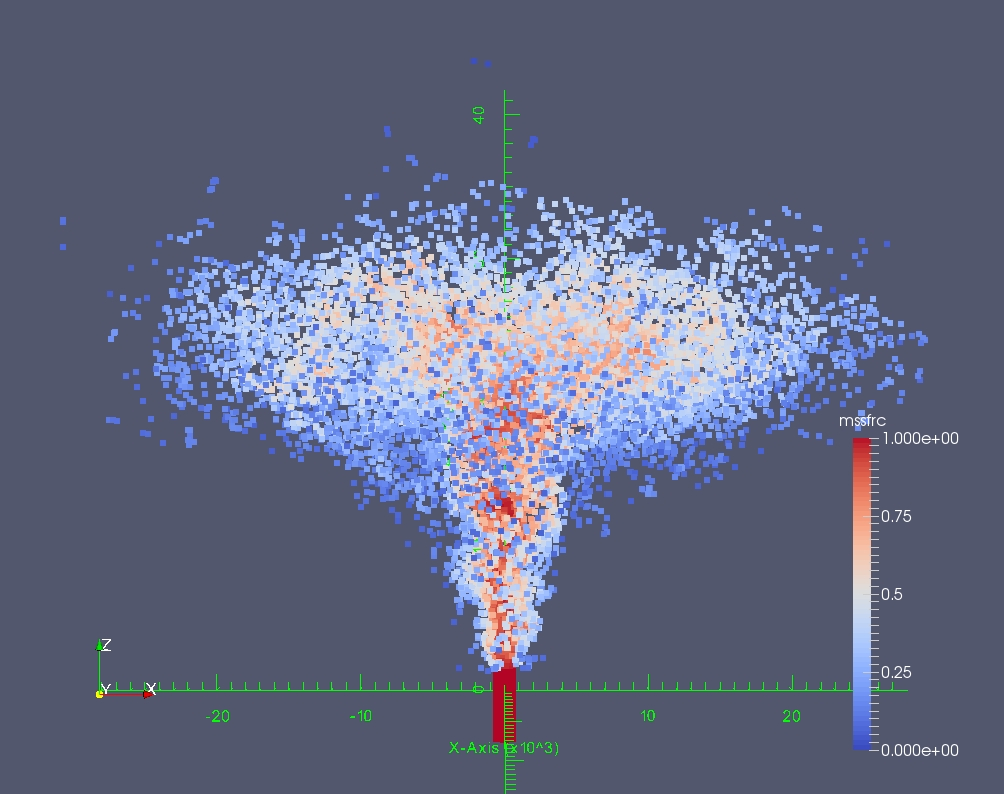
\includegraphics[width=0.99 \textwidth]{Chapter-7/Figures/mssfrc_front-filter-by-phase}
    \end{minipage}%
    \begin{minipage}{.325 \textwidth}
        \centering
        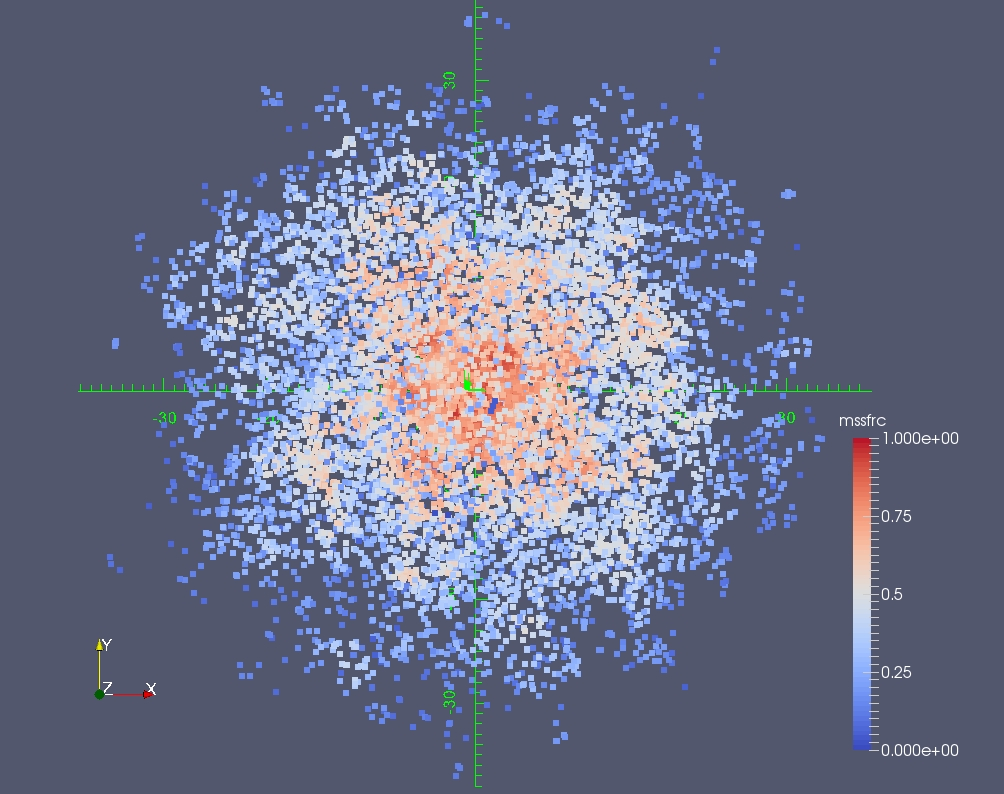
\includegraphics[width=0.99 \textwidth]{Chapter-7/Figures/mssfrc_top-with-axis}
    \end{minipage}%
    \begin{minipage}{.325 \textwidth}
        \centering
        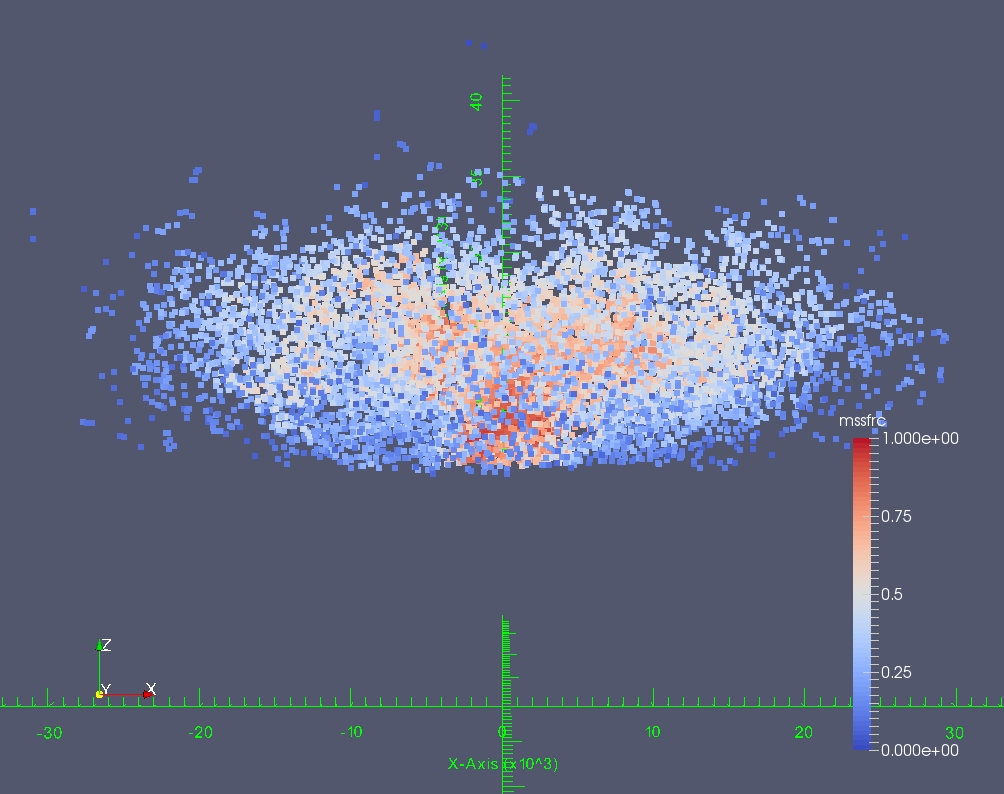
\includegraphics[width=0.99 \textwidth]{Chapter-7/Figures/mssfrc_front-z15000}
    \end{minipage}%   
    \caption{The Pinatubo plume simulated by Plume-SPH. Red represents high mass fraction of erupted material while blue represents low mass fraction. All particles in the pictures are of type phase 2 (SPH particles that represent erupted material) at 600s after eruption, at which time, the plume has already reached the steady state and started spreading radially. The radially expanding portion of the plume are extracted as initial ash cloud. Pictures from left to right are: front view of the whole plume, top view of the plume and front view of the initial ash cloud, which is essentially portion of the whole plume with elevation higher than a given threshold (in this picture is $15000 m$)}
    \label{fig:Plume-SPH-Pinatubo-ash-cloud}
\end{figure}

Table \ref{tab:VATDs-source-term-determination} compares three different manners for creating initial conditions for VATDs: creating initial ash cloud without any plume model, creating initial ash cloud based on output of 1D plume model and extracting initial ash cloud from 3D plume simulation. The first method determines all parameters by calibration. Then create initial ash cloud according to semiempirical plume shape expression. Other two methods both depend on plume models. Compared with 3D plume models, even though 1D plume models also accounting for basic conservation laws, requires calibration of entrainment coefficients. What's more, 3D plume model can generate an initial ash cloud in a 3D space while 1D plume assumes a specific plume shape (such as Poisson or Suzuki). In addition, the number of particles in the first two manners for generating initial ash cloud is free parameter while it depends on simulating in the third manner. 
 
\begin{table}[htp]
\centering
      \caption{Three different manners for determining input parameters that define the initial ash clouds for PUFF simulation}		
	  \begin{tabular}{p{19mm}p{23mm}p{20mm}p{20mm}p{20mm}p{20mm}p{18mm}}
	    \hline
	          & Maximum \newline height & Average \newline height & Vertical \newline spread & Column \newline radius & Plume \newline shape & number \newline of particles\\
	    \hline
	    No model & Observation $\&$ \newline Calibration & Calibration & Calibration & Calibration & Semiempirical & Free \newline parameter \\
	    bent (1D) & Semiempirical & Conservation \newline laws (1D) & Semiempirical & Conservation \newline laws (1D) & Semiempirical & Free \newline parameter\\
	    Plume-SPH \newline (3D) & 1st principle & 1st principle & 1st principle & 1st principle & 1st principle & Based on \newline simulation \\
	    \hline
	  \end{tabular}
	  \label{tab:VATDs-source-term-determination}
\end{table}

\subsection{Sensitivity of other parameters}

Besides initial parameters, other input parameters for PUFF simulation are: horizontal diffusivity, vertical diffusivity, mean grain size, grain size standard deviation, particles' number and eruption duration. We present in this section determination of eruption duration and sensitivity studies on other parameters.

The plume development and ash transportation are of different time scale and length scale.
It takes around 600s for Pinatubo plume to reach the steady state. However the duration of climactic phase of eruption might persist for a few hours (9 hours in our case study). It is computationally too expensive to do 3D plume simulation for several hours. To handle these difficulties, we restart PUFF at an interval of $600 s$. At every restart, we integrate the output of PUFF of the last simulation with the ash cloud obtained from output of Plume-SPH. In this way, the persistent eruption is mimicked by pulse releasing of ash clouds. The interval of the pulse release equals to the simulation time of plume model, that is $600 s$ in our case study. The total number of particles used in PUFF equals to summation of particles in all these releases. The number of particles in each ash clouds depends on plume simulation, and the total number of releases depends on eruption duration. So the number of particles is not a parameter selected by user any more.

A systematic sensitivity study is applied to check how other input parameters would influence the simulation results. Such sensitivity analyses will serve as basis for identifying possible sources of disparities between simulation and observation.
The sensitivity analyses illustrate that adjustment of other input parameters produces negligible visual differences in ash cloud distribution. Using different vertical diffusivities in range of $[100, 100000] m^2s^{-1} $ and different horizontal diffusivities in range of $[1, 20] m^2s^{-1}$ produces visually negligible differences, too. 
The eruption duration should depend on the actual eruption duration (or the duration of climactic phase) of a specific eruption. We conducted several simulations with eruption duration varying in range of $[5, 11] hours$ with slight different starting time of climactic phase. Table \ref{tab:sensitivity-start-end-time} lists all these simulations. However, only tiny visible differences are observed among the simulated ash distributions. The mean of grain size also has visually ignorable effects on long-term ash distribution according to our sensitivity tests varying the log mean (base 10) grain radius in a range of $[-7.3, -3.5] m$. 
%When using extreme small mean grain size, PUFF is supposed to forecast transportation of volcanic gases. 
The standard deviation, when varying in range of $[0.1, 10]$, also generate ignorable difference on long-term ash distribution. Similar conclusion on parameter sensitivity is reported by \citet{fero2008simulation}.
Among these parameters, the eruption duration and beginning time shows, even though tiny, the most obvious influence on simulated ash distribution. In order to show such differences in an intuitive way, Fig. \ref{fig:PUFF-sensitivity-duration} shows ash distribution corresponding to 4.9 hours duration, 9 hours duration and 11 hours duration respectively. After 72 hours, relative to the simulation starting time, these three cases generate generally similar result, with high concentration ash covers almost the same region. The difference of lower concentration distribution is relatively more obvious. Simulated volcanic ash covers broadest area when eruption duration is 11.1 hours. To summarize, all other input parameters have either tiny or ignorable affects on long-term ash distribution simulation. 

\begin{table}[htp]
\centering
      \caption{The starting and ending time (UT) for simulating the climactic phase of Pinatubo eruption on June 15 1991.}		
	  \begin{tabular}{p{45mm}p{23mm}p{23mm}p{23mm}p{23mm}}
	    \hline
        Eruption duration & 4.9 hours & 9 hours & 10 hours & 11.1 hours \\
	    \hline
	    Start Time & 0441 & 0441 & 0441 & 0334 \\
	    	Observed height at the start & 37.5 km & 37.5 km  & 37.5 km  & 24.5 km \\
	    
	    End time   & 0934 & 1341 & 1441 & 1441  \\
	    		Observed height at the end & 35 km & 26.5 km & 22.5 & 22.5 km \\
	    \hline
	  \end{tabular}
	  \label{tab:Pinatubo-eruption-duration}
\end{table}

\begin{figure}[!htb]
    \centering
    \begin{minipage}{.325\textwidth}
        \centering
        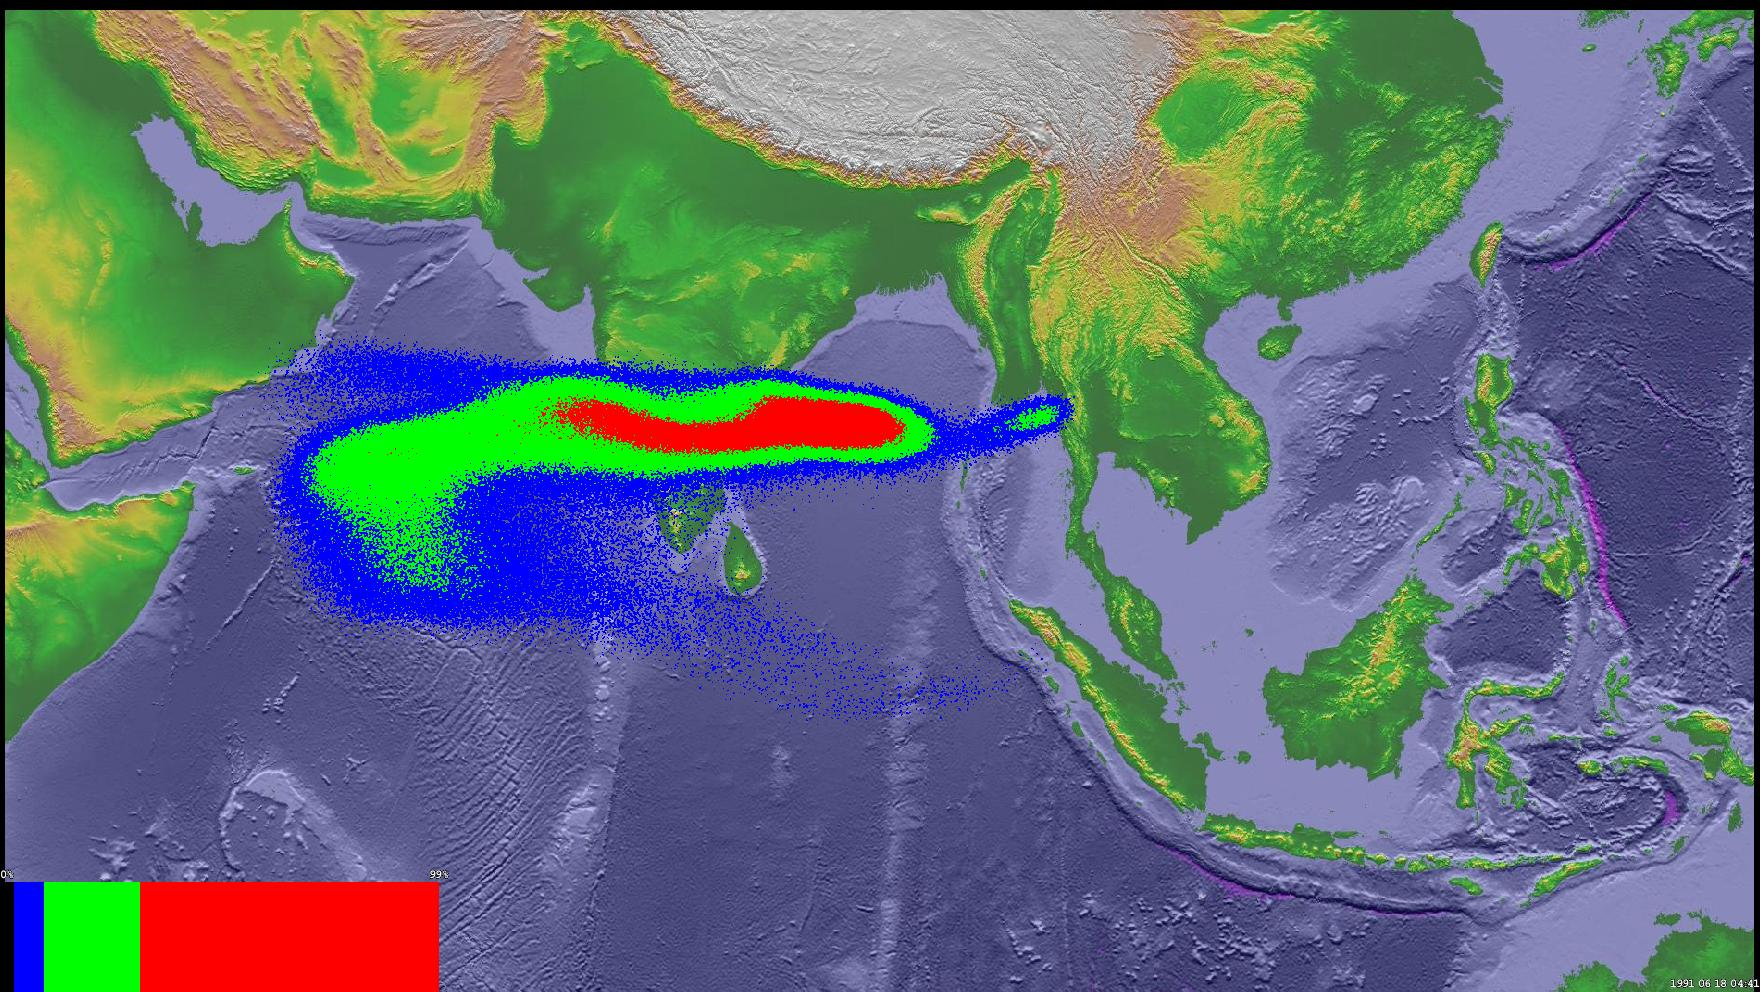
\includegraphics[width=0.99 \textwidth]{Chapter-7/Figures/199106180441-ash-5hr-cut15000}
    \end{minipage}%
    \begin{minipage}{.325 \textwidth}
        \centering
        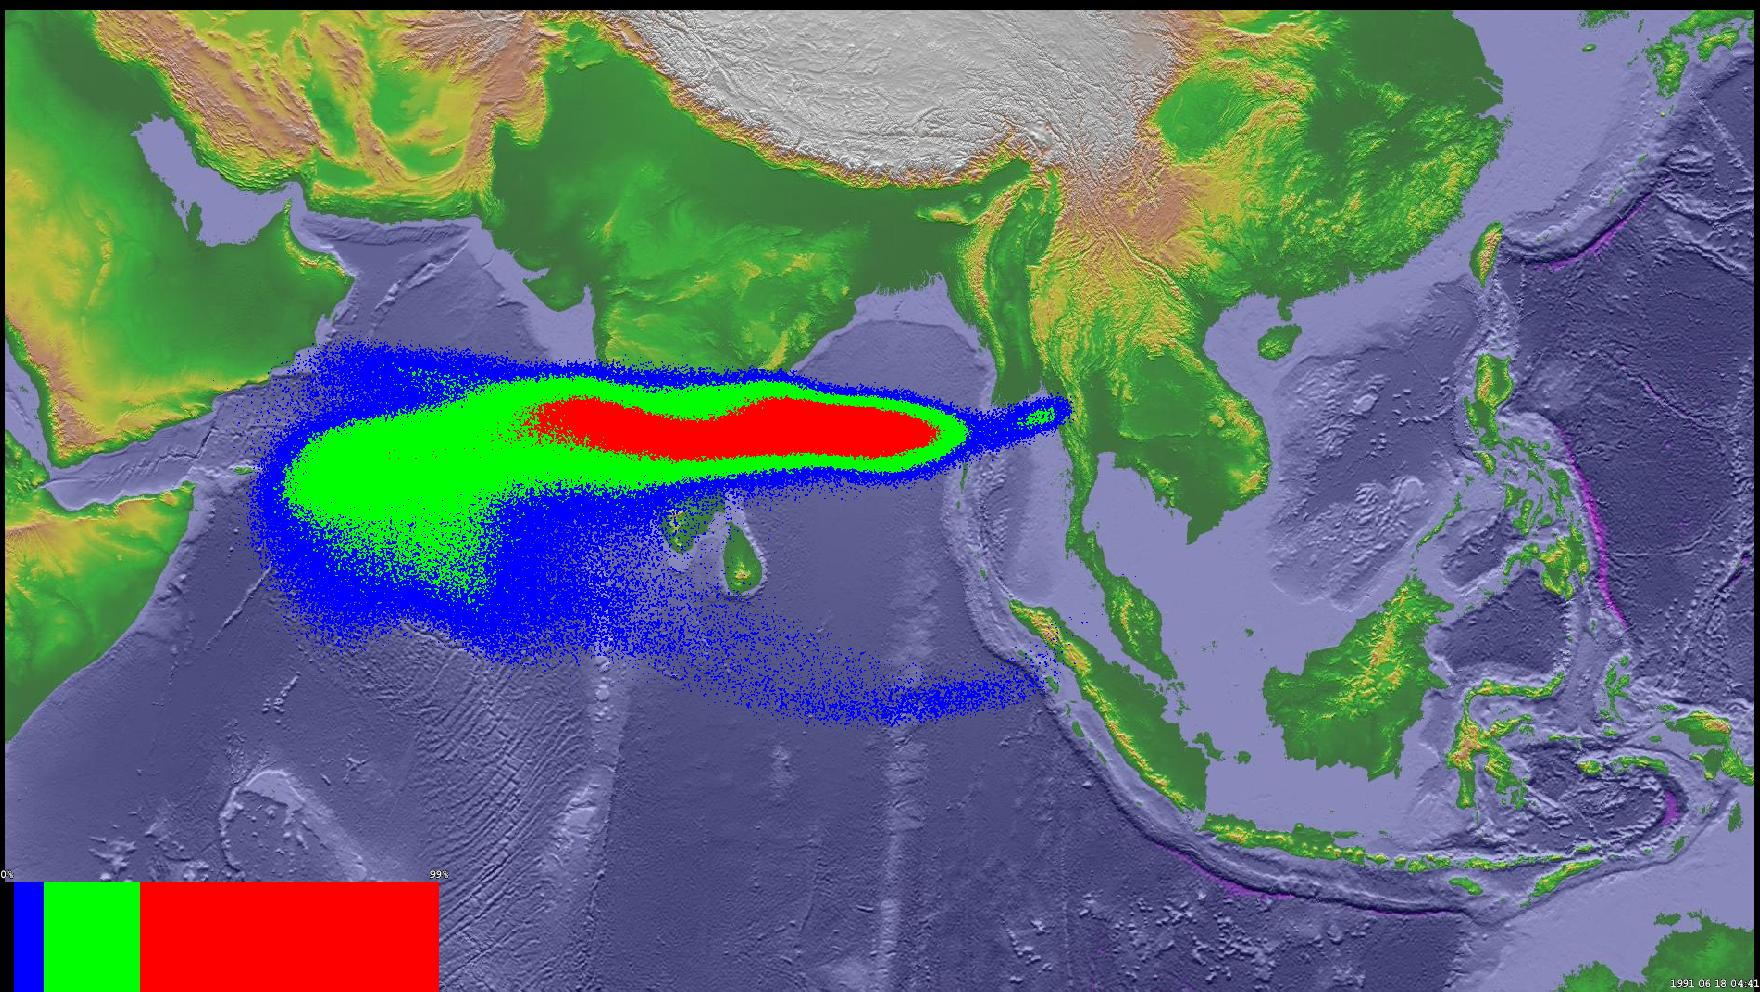
\includegraphics[width=0.99 \textwidth]{Chapter-7/Figures/199106180441-ash-9hr-cut15000}
    \end{minipage}%
    \begin{minipage}{.325 \textwidth}
        \centering
        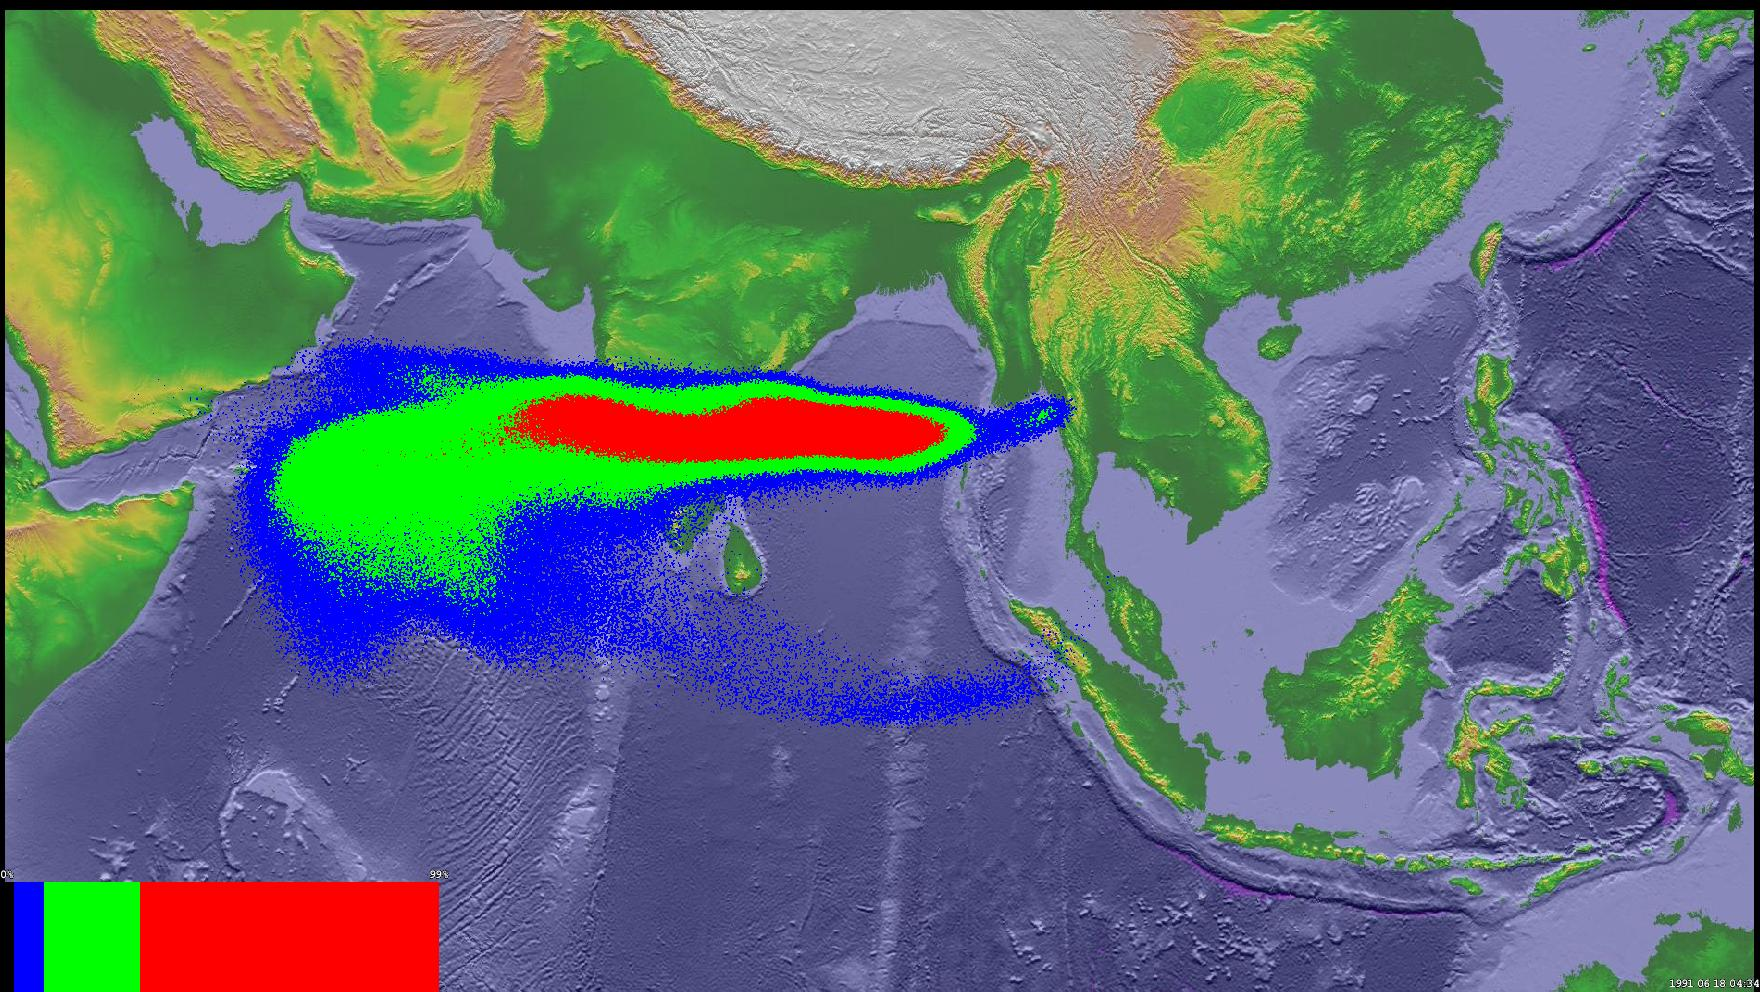
\includegraphics[width=0.99 \textwidth]{Chapter-7/Figures/199106180441-ash-11hr-cut15000}
    \end{minipage}%   
    \caption{Simulated ash cloud distribution corresponding to eruption duration of 4.9 hours, 9 hours and 11.1 hours (from left to right) respectively. Starting and ending time for each case is in Table \ref{tab:VATDs-source-term-determination}. The contours are for ash distribution at 72 hours after eruption.}
    \label{fig:PUFF-sensitivity-duration}
\end{figure}

The new methodology of generating initial ash cloud introduces another new parameter: elevation threshold. We also carry out sensitivity analysis on this parameter by varying the elevation threshold from $1500 m$ (the height of the vent) to $25000 m$. The simulated ash distributions show obviously visible differences. Such influence is especially obvious when the elevation threshold is either very large or very small. However, varying the elevation threshold in the range of $[12000, 18000] m$ generates relatively small difference in ash distribution. Figure \ref{fig:PUFF-sensitivity-elevation-threshold} compares the simulated ash distribution corresponding to elevation thresholds of $1500 m$ and $15000 m$. Compared with ash distribution for threshold of  $15000 m$, an extra long tail appears when using elevation threshold of $1500 m$. Adopting smaller elevation thresholds essentially adds more tracers at lower elevation. As the direction of wind at different elevation are different, these newly added tracers at lower elevation would transpose to different directions.

\begin{figure}[!htb]
    \centering
    \begin{minipage}{.325\textwidth}
        \centering
        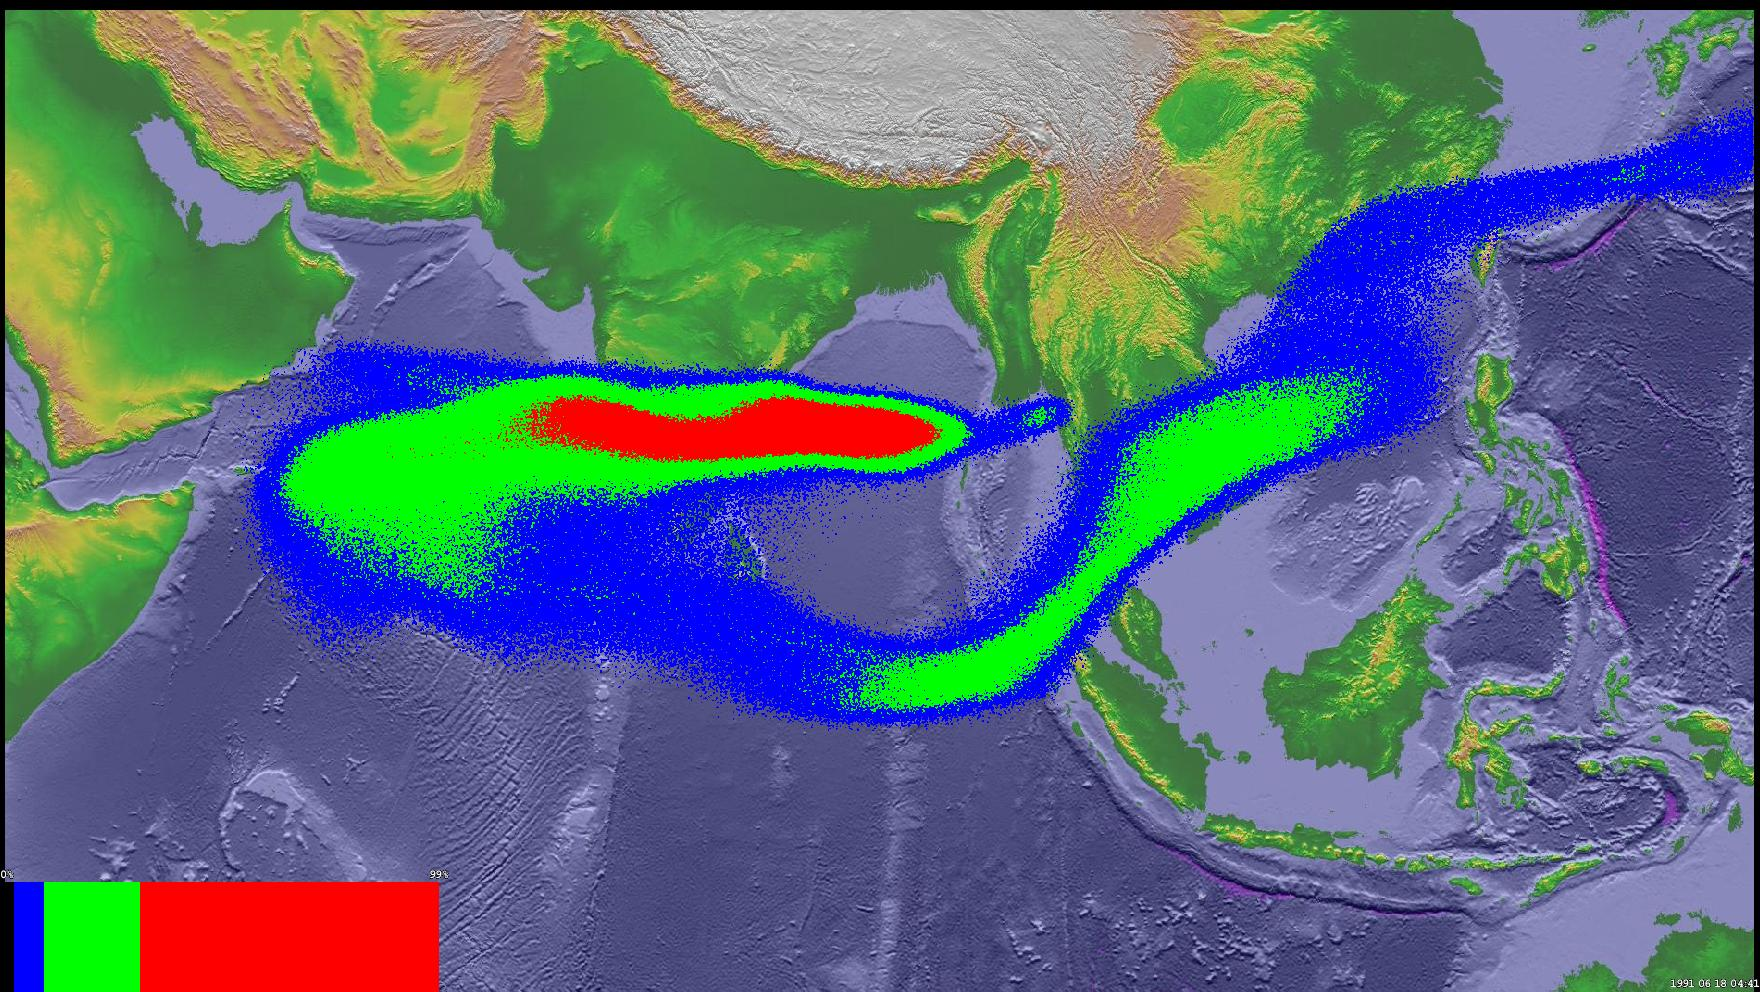
\includegraphics[width=0.99 \textwidth]{Chapter-7/Figures/199106180441-ash-9hr-cut1500}
    \end{minipage}%
    \begin{minipage}{.325 \textwidth}
        \centering
        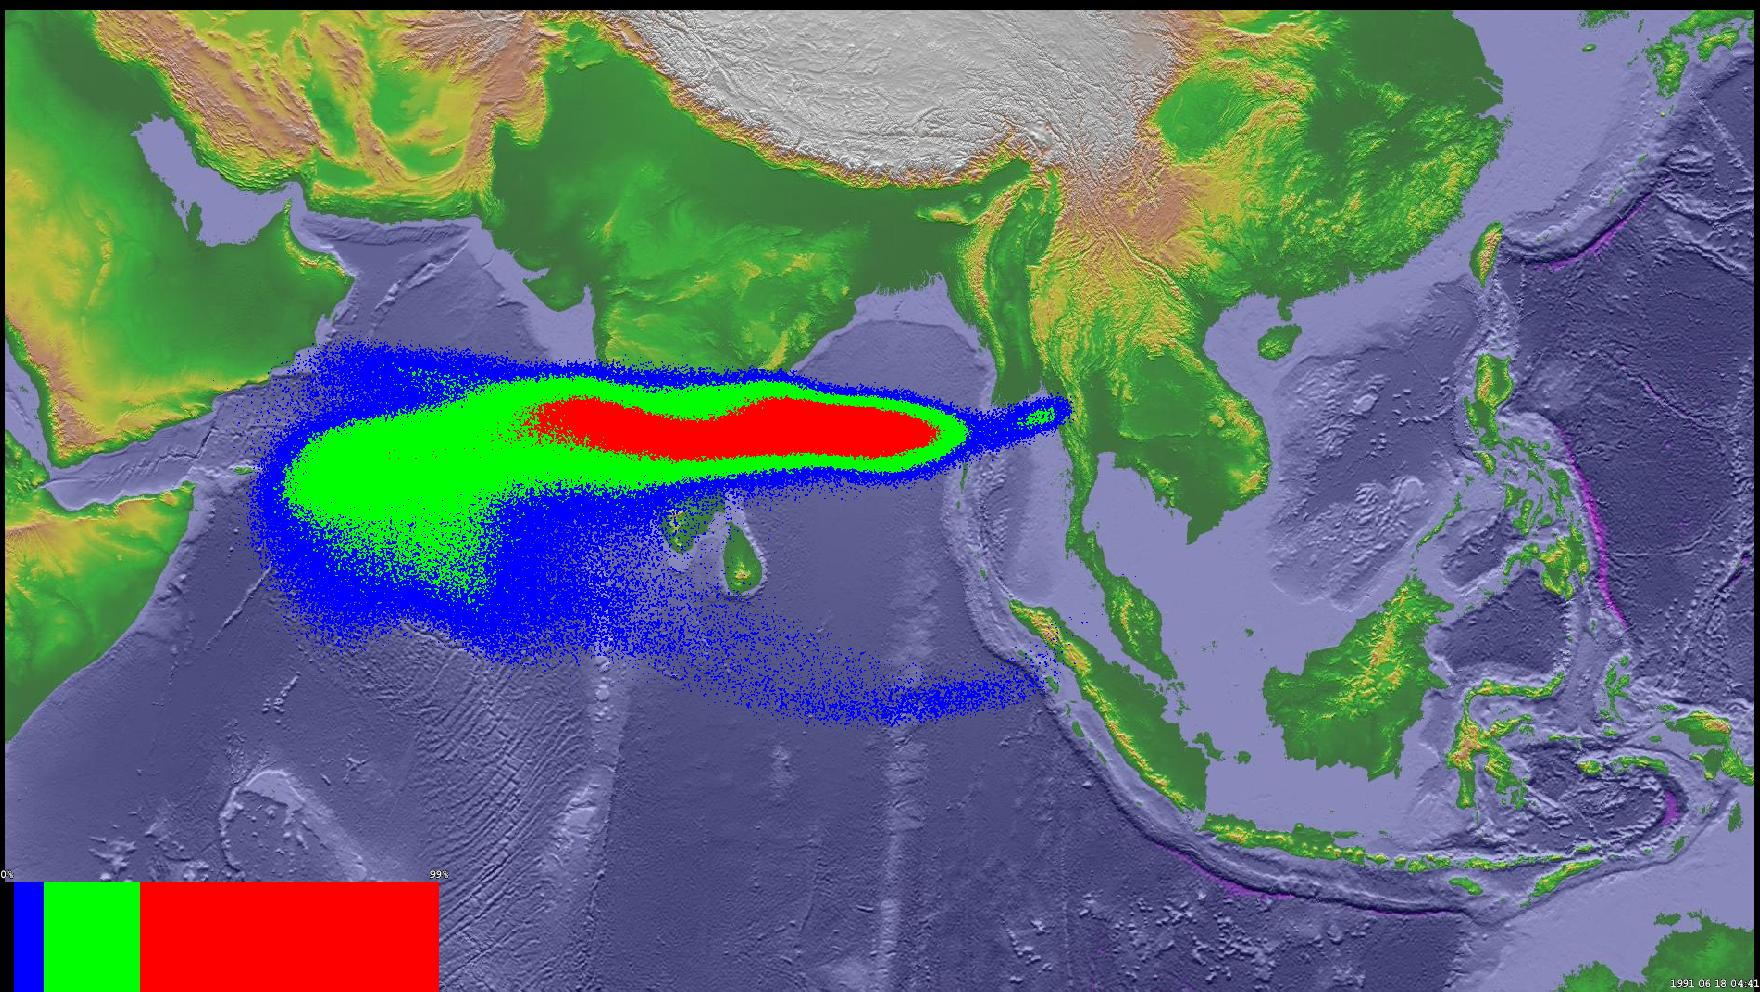
\includegraphics[width=0.99 \textwidth]{Chapter-7/Figures/199106180441-ash-9hr-cut15000}
    \end{minipage}%  
    \caption{Simulated ash distribution taking initial ash clouds obtained using different elevation thresholds ($1500 m$ and $15000$ m) from output of Plume-SPH. The contours are corresponding to ash concentration at 72 hours after eruption. The starting and ending time are corresponding to 9 hours case in Table \ref{tab:Pinatubo-eruption-duration}}
    \label{fig:PUFF-sensitivity-elevation-threshold}
\end{figure}

The sensitivity analyses demonstrate that the initial ash cloud, or the initial condition for VATDs has the most significant effect on simulated ash distribution while all other input parameters have either tiny or ignorable influence. The initial ash cloud generated based on semiempirical expression, which is a function of several parameters, might be significantly disparate from realistic ash cloud. Such initial condition might greatly compromise the accuracy of PUFF simulation.

\section{Results and discussion}

Ash distribution are simulated based on initial parameters generated by 1D plume simulation (bent) and initial ash cloud extracted from 3D plume simulation (Plume-SPH). The maximum height is then adjusted manually to obtain best match ash distribution. The results are compared against observational ash clouds to evaluate the accuracy of each simulation. To identify the source of disparity between simulation and observation of long-term ash transportation, PUFF simulation results are also compared against observed $SO_2$ clouds.

%\begin{table}[htp]
%	\centering
%      \caption{List of eruption condition and material properties for plume simulation}		
%	  \begin{tabular}{lrr}
%	    \hline
%	    Parameters & Units & Plume \\
%	    \hline
%	    Vent velocity          & $m\cdot s^{-1}$  & 275 \\
%	    Vent gas mass fraction &                  & 0.05 \\
%	    Vent Temperature       & $K$              & 1053 \\
%	    Vent height            & $m$              & 1500 \\
%	    Mass discharge rate    & $kg\cdot s^{-1}$ & $1.5 \times 10^9$\\
%	    	Specific heat of gas at constant volume     & $J \cdot kg^{-1}\cdot K^{-1}$ & 717     \\
%	    Specific heat of air at constant volume     & $J \cdot kg^{-1}\cdot K^{-1}$ & 1340    \\
%	    	Specific heat of solid                      & $J \cdot kg^{-1}\cdot K^{-1}$ & 1100    \\
%	    	Specific heat of gas at constant pressure   & $J \cdot kg^{-1}\cdot K^{-1}$ & 1000    \\
%	    	Specific heat of air at constant pressure   & $J \cdot kg^{-1}\cdot K^{-1}$ & 1810    \\
%	    	Density of air at vent height               & $kg \cdot m^{-3}$       & 1.104   \\
%	    Pressure at vent height                     & $Pa$                    & 84363.4 \\
%	    \hline
%	  \end{tabular}
%	  \label{tab:input_parameters_plume_simulation}
%\end{table}

%Eruption parameters, material properties and atmosphere for both plume simulations are the same. Parameters for the strong plume no wind case in a comparison study on eruptive column models \citep {costa2016results} are adopted. Eruption conditions and material properties are listed in Table \ref{tab:input_parameters_plume_simulation}. Note that the density of erupted material at the vent and radius of the vent can be computed from the given parameters. The eruption pressure is assumed to be as the same as pressure of ambient at the vent and hence is not given in the table. The vertical profiles of atmospheric properties were obtained based on the reanalysis data from ECMWF (European Centre for Medium-Range Weather Forecasts) for the period corresponding to the climactic phase of the Pinatubo eruption.

The plume development simulation are described in detail in Chapter 6. 1D plume simulation using bent adopts exactly the same eruption parameters, material properties and atmosphere as Plume-SPH (Table \ref{tab:material_properties}, Table \ref{tab:input_parameters}).
For ash transportation simulation, initial condition is defined based on plume simulation output. Two parameters obtained directly from bent simulation, the horizontal spread and height of plume, are used to define the initial ash cloud together with several other parameters assigned semiempirically \citep{bursik2012estimation}. See details in Table \ref{tab:input_parameter_PUFF_simulation}. The output of Plume-SPH is a group of SPH particles in 3D space, from which the initial ash cloud can be directly extracted based on an elevation threshold without using any other parameters. The simulation parameters which control the simulation characteristics are the same for both simulations. As has been shown in sensitivity analyses section, these parameters have less influence on simulation results compared with initial condition. Details can be found in Table \ref{tab:input_parameter_PUFF_simulation}.

\begin{table}[htp]
\centering
      \caption{Other parameters for PUFF simulation of the climactic phase of Pinatubo eruption on June 15 1991. The first six parameters define the initial condition. The first four parameters for bent are based on plume modeling.}	
	  \begin{tabular}{lrrr}
	    \hline
	    Parameters    & Unit & Bent & Plume-SPH \\
	    \hline
	    Maximum Height & $m$ & 41343.9 & - \\
	    Minimum Height & $m$ & 28019.7 & - \\
	    Horizontal Spread & $km$ & 103.808 & -\\
	    Vertical Spread & $km$ & 6.662  & - \\
	    Plume Shape & - & Poisson & - \\
	    Total Ash Particles  & - & 1768500 & - \\
	    Elevation Threshold & $m$ & - &  15000 \\
	    Horizontal Diffusivity & $m^2/s$ &10000 & 10000\\
	    Vertical Diffusivity & $m^2/s$ & 10 & 10 \\
	    Grain Size Distribution & - & Gaussian & Gaussian  \\
	    Mean of Grain Size (Radius) & $mm$ & $3.5 \times 10 ^-2$ & $3.5 \times 10 ^-2$ \\
	    Standard Deviation of Grain Size & - &  1.0 & 1.0 \\
	    	Start Time & UT & 0441 & 0441 \\
	    End time & UT & 1341 & 1341 \\
	    Simulation Duration & hr & 120 & 120 \\
	    \hline
	  \end{tabular}
	  \label{tab:input_parameter_PUFF_simulation}
\end{table}

\subsection{``Plume-SPH+PUFF" and ``bent+PUFF"}

Simulation results based on input parameters list in Table \ref{tab:input_parameters}, Table \ref{tab:material_properties} and Table \ref{tab:input_parameter_PUFF_simulation} are compared with TOMS images and AVHRR BTD ash cloud map in Fig. \ref{fig:Plume-SPH-PUFF-ash-cloud}.

\begin{figure}[!htb]
    \centering
    \begin{minipage}{.325\textwidth}
        \centering
        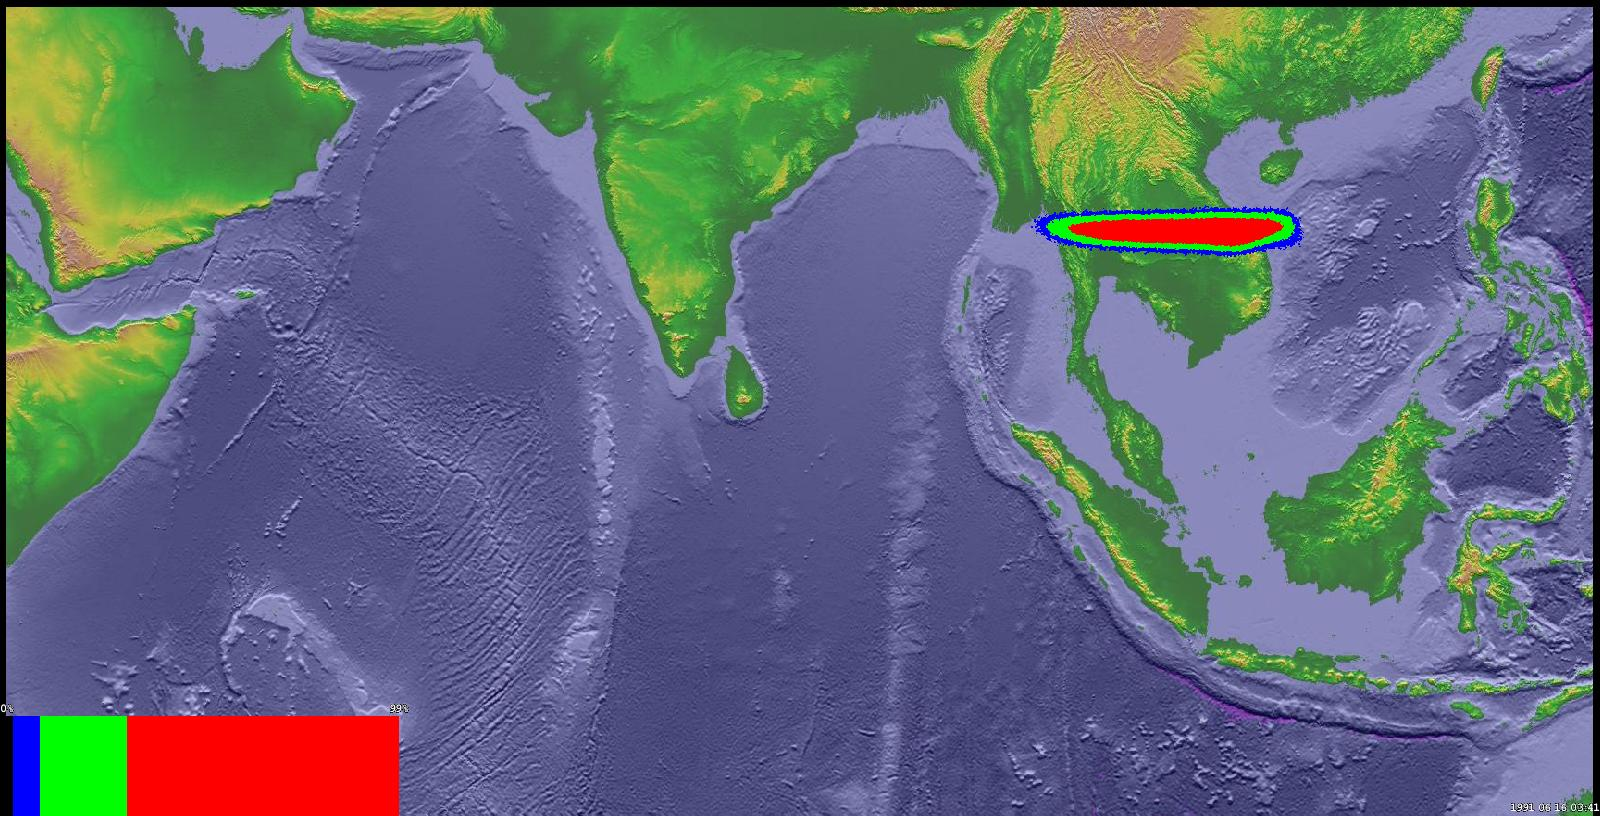
\includegraphics[width=0.99 \textwidth]{Chapter-7/Figures/bent-23hr-ash}
    \end{minipage}%
    \begin{minipage}{.325 \textwidth}
        \centering
        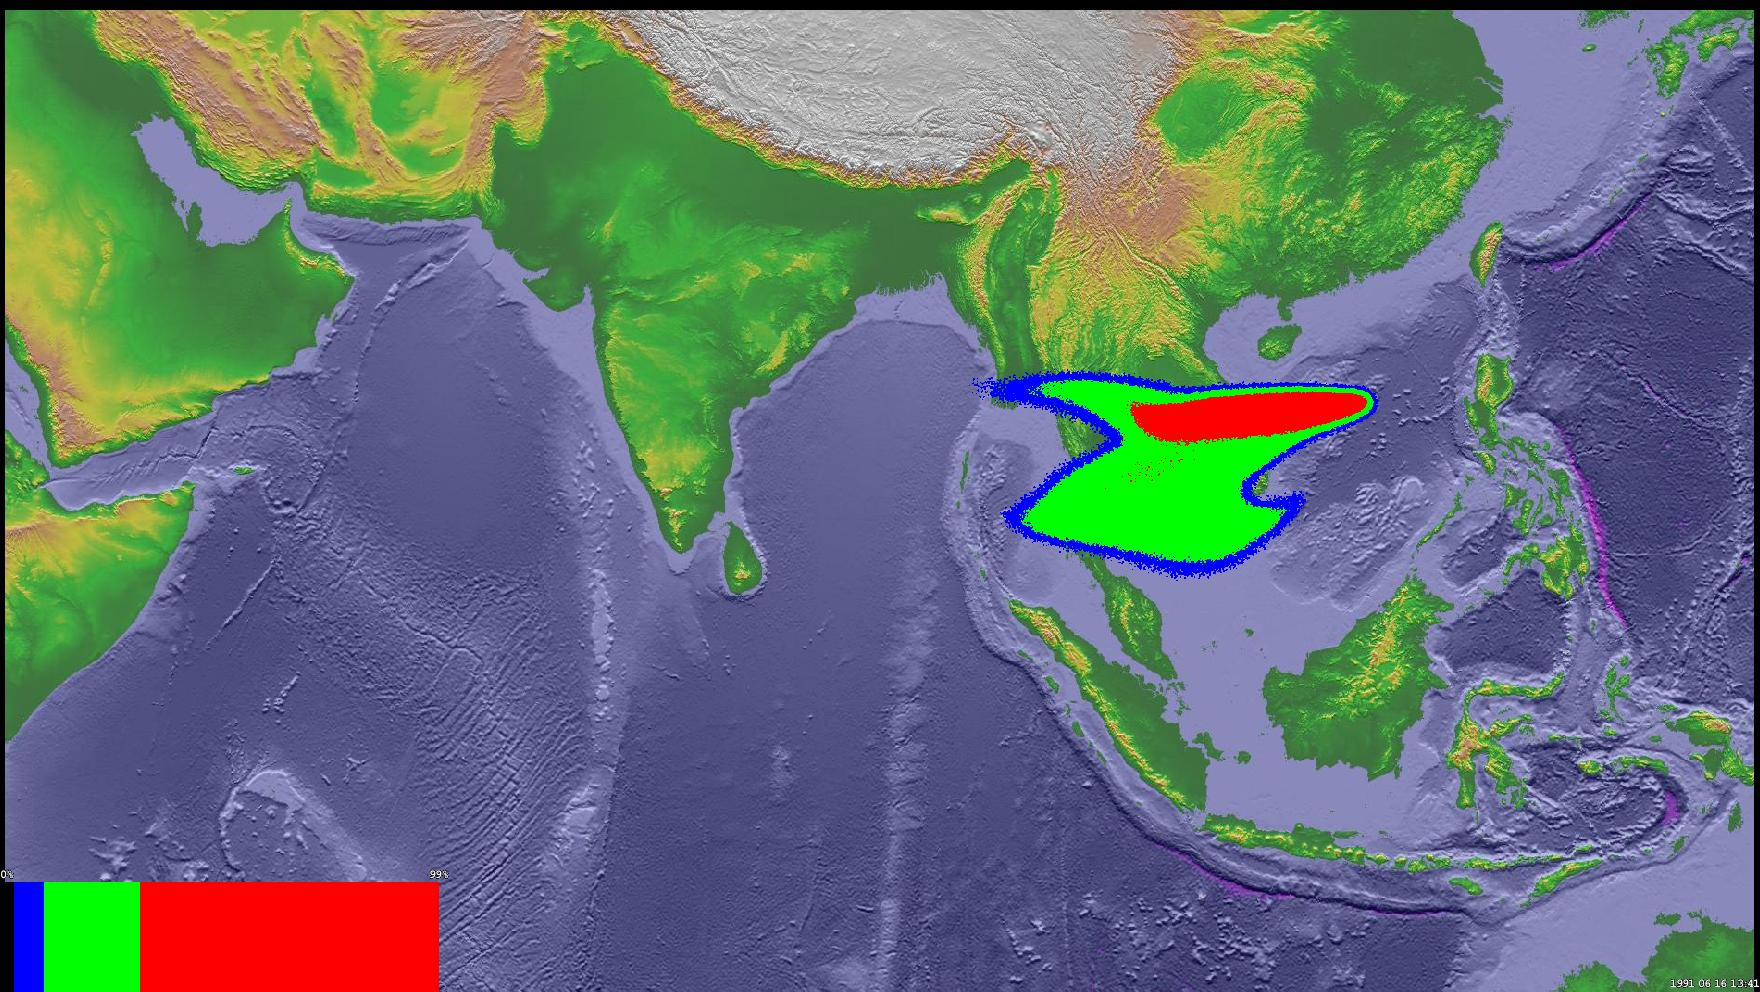
\includegraphics[width=0.99 \textwidth]{Chapter-7/Figures/SPH-Plume-23hr-ash}
    \end{minipage}%
    \begin{minipage}{.325 \textwidth}
        \centering
        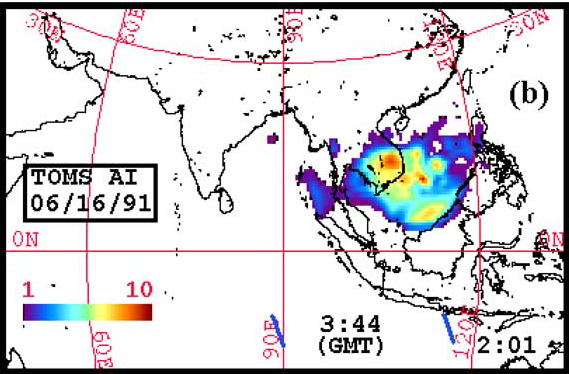
\includegraphics[width=0.99 \textwidth]{Chapter-7/Figures/OB-ash-23hr-ash}
    \end{minipage}% 
    \\
        \begin{minipage}{.325\textwidth}
        \centering
        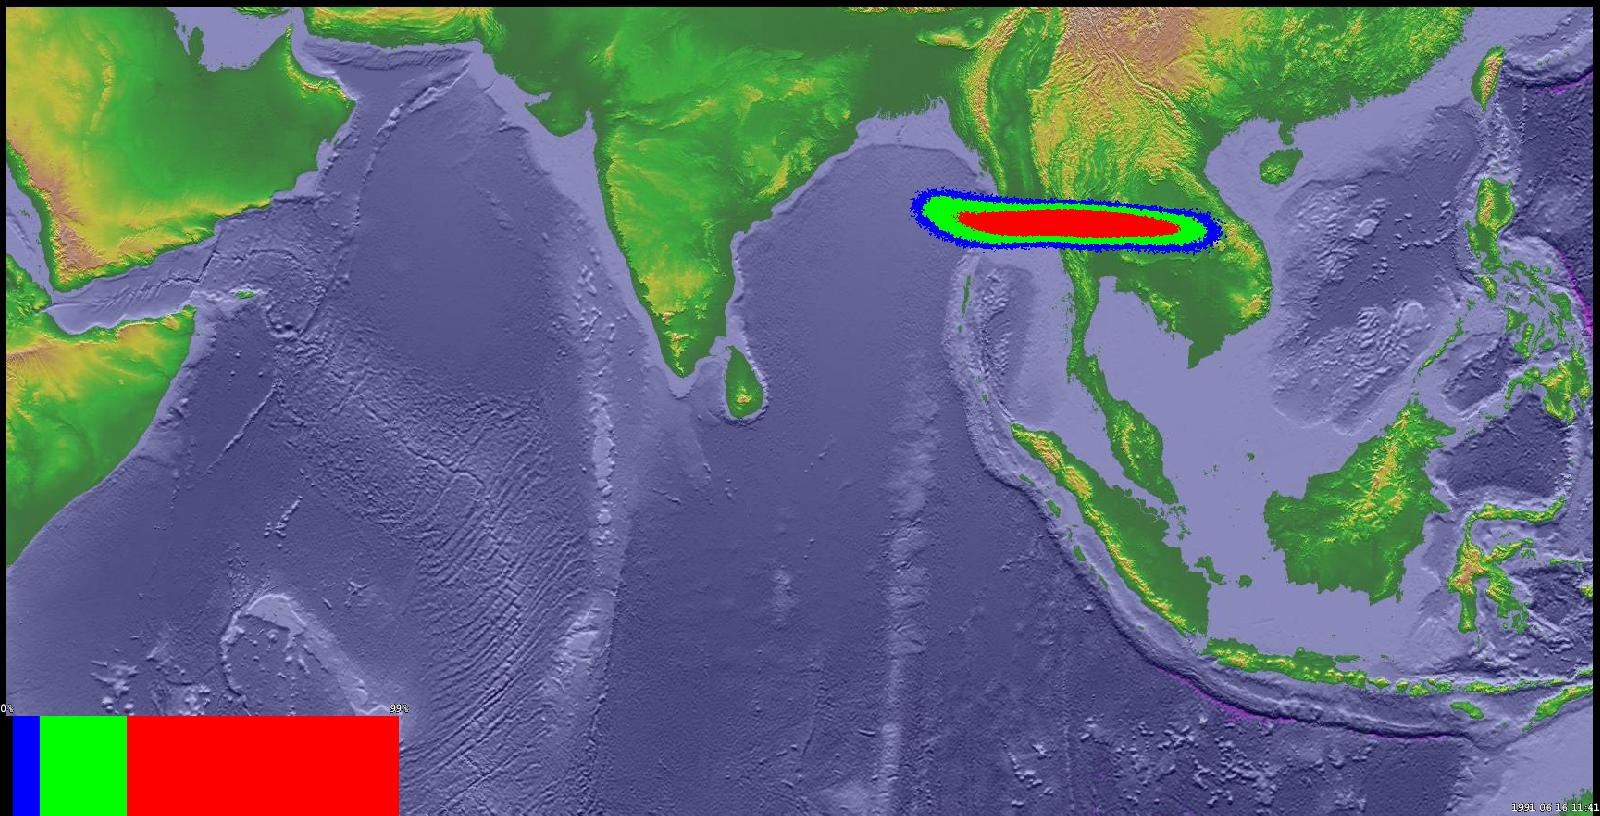
\includegraphics[width=0.99 \textwidth]{Chapter-7/Figures/bent-31hr-ash}
    \end{minipage}%
    \begin{minipage}{.325 \textwidth}
        \centering
        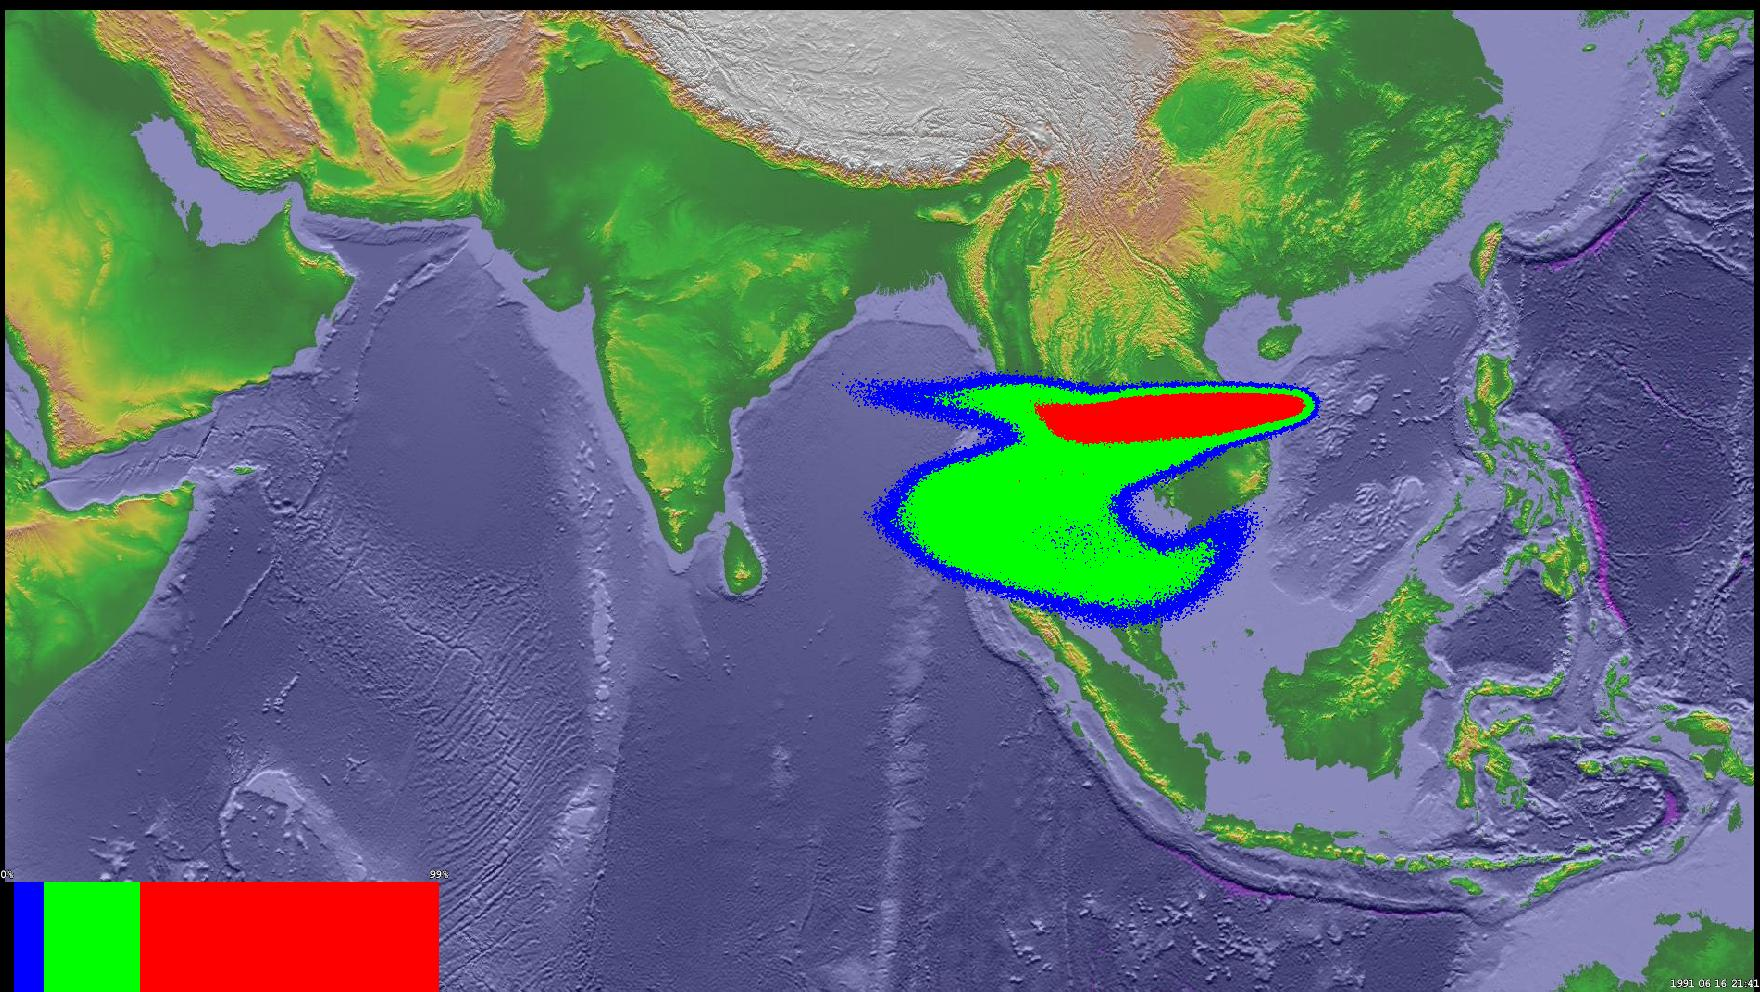
\includegraphics[width=0.99 \textwidth]{Chapter-7/Figures/SPH-Plume-31hr-ash}
    \end{minipage}%
    \begin{minipage}{.325 \textwidth}
        \centering
        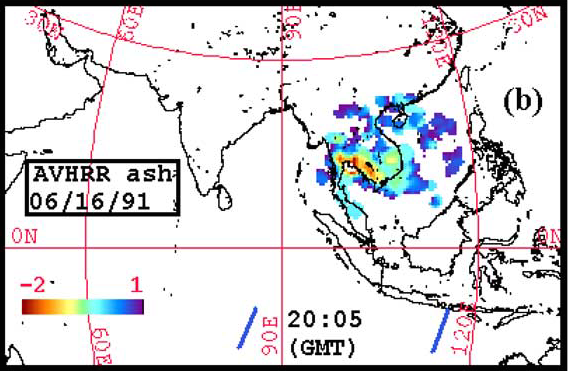
\includegraphics[width=0.99 \textwidth]{Chapter-7/Figures/OB-ash-31hr-ash}
    \end{minipage}% 
    \\
        \begin{minipage}{.325\textwidth}
        \centering
        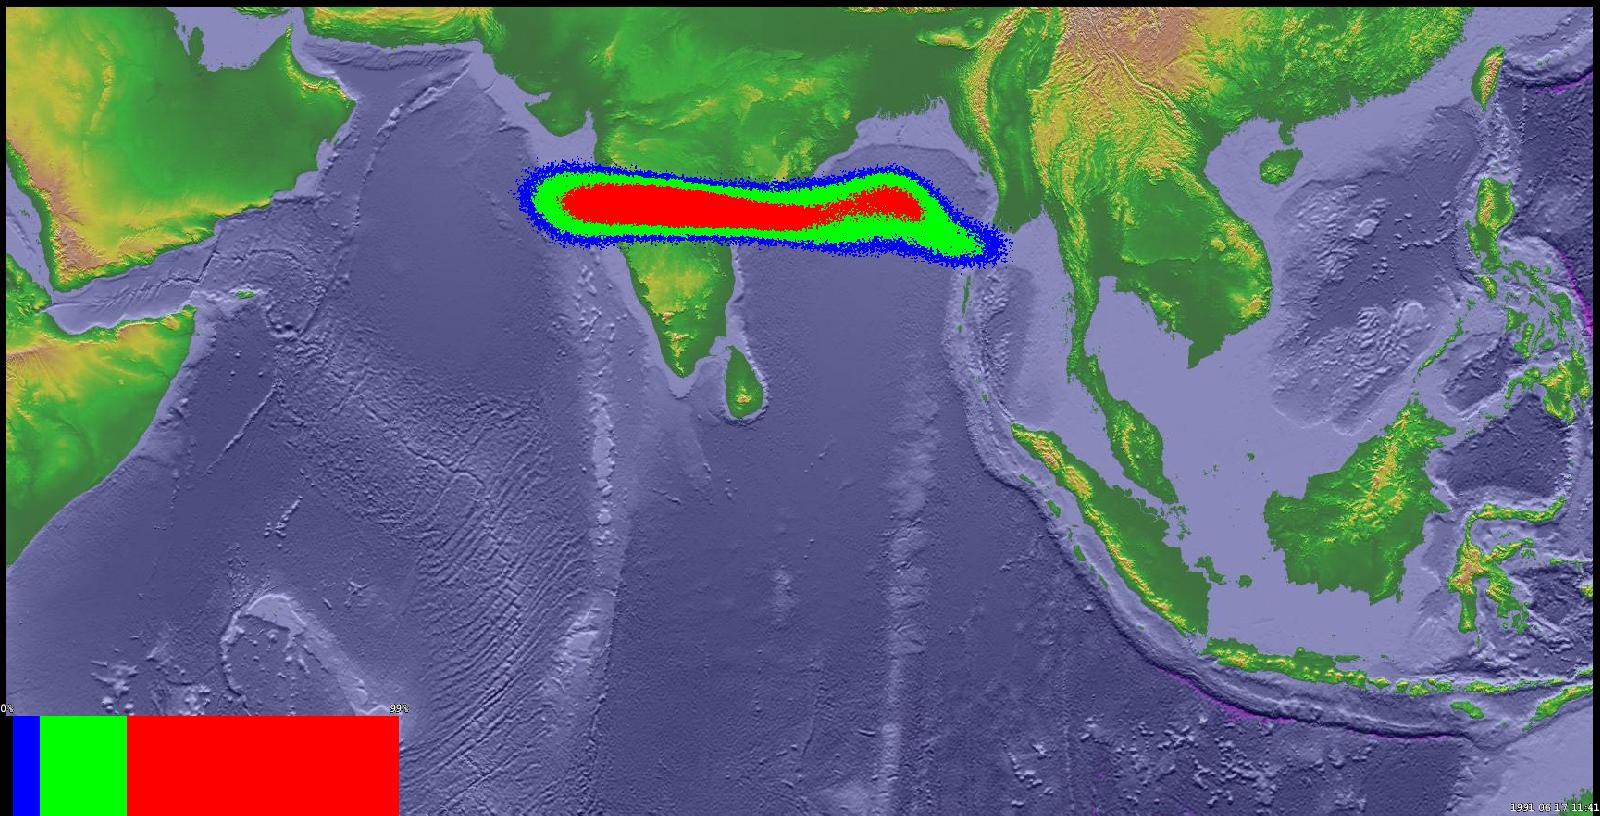
\includegraphics[width=0.99 \textwidth]{Chapter-7/Figures/bent-55hr-ash}
    \end{minipage}%
    \begin{minipage}{.325 \textwidth}
        \centering
        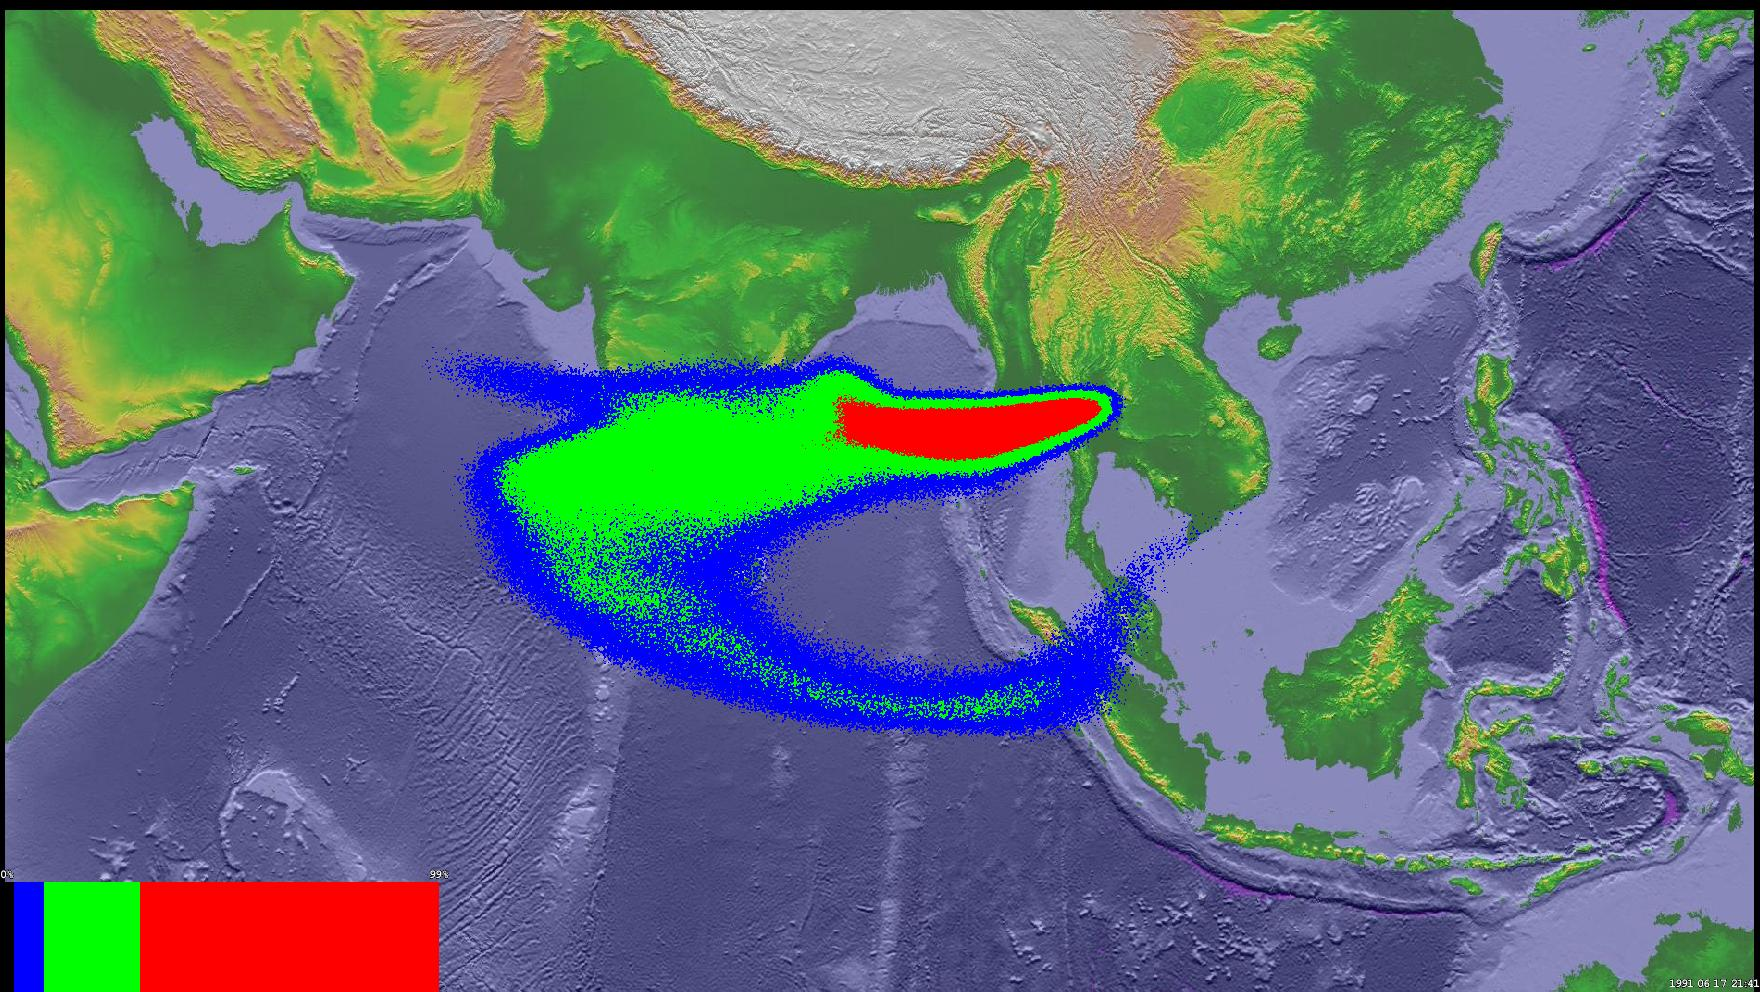
\includegraphics[width=0.99 \textwidth]{Chapter-7/Figures/SPH-Plume-55hr-ash}
    \end{minipage}%
    \begin{minipage}{.325 \textwidth}
        \centering
        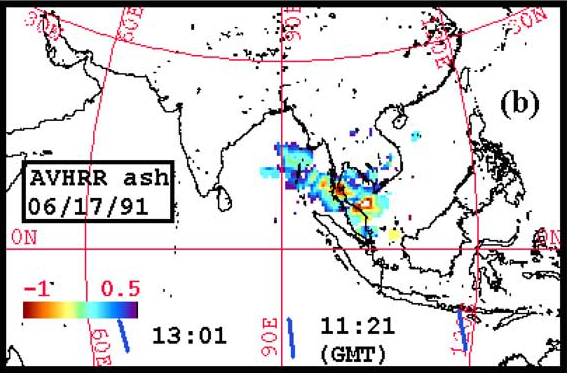
\includegraphics[width=0.99 \textwidth]{Chapter-7/Figures/OB-ash-55hr-ash}
    \end{minipage}% 
    \caption{Comparison of ``bent+PUFF" and ``Plume-SPH+PUFF" simulation results. Pictures from left to right are: PUFF simulation based on bent, PUFF simulation based on Plume-SPH, TOMS or AVHRR image of Pinatubo ash cloud. Ash clouds at different hours after eruption are on different rows. From top to bottom, the images are corresponding to around 23 hours after eruption (UT 199106160341), 31 hours after eruption (UT 199106161141), 55 hours after eruption (UT 199106171141). The observation data on the first row are TOMS ash and ice map. The observation data on the second and third row are AVHRR BTD ash cloud map with atmospheric correction method applied.}
    \label{fig:Plume-SPH-PUFF-ash-cloud}
\end{figure}

The difference in simulation results between ``bent+PUFF" and ``Plume-SPH+PUFF" is obvious. The simulated ash distribution based on initial condition created from Plume-SPH is much closer to observation than that based on bent. Around 23 hours and 31 hours after the beginning of the climactic phase, ``Plume-SPH+PUFF" simulation generates ash images that generally close to observational image, especially the location where the high concentration ash presents. However, these ash at near west to Pinatubo mountain observed in satellite images does not present in ``Plume-SPH+PUFF" simulation results. This disparity is very possible due to the fact that the Pinatubo eruption continued after climactic phase while our simulation only simulates the climactic phase. The ash released after climactic phase is not accounted in the simulation results. The ``bent+PUFF" simulation, however, forecasts an ash distribution faster and narrower than observation. The location, where the high concentration ash presents, locates to the northwest of observed ash. 
Around 55 hours after the beginning of the climactic phase, the disparity between observation and simulation becomes more obvious. Ash distribution of ``bent+PUFF" simulation locates far west to the observed ash. The high concentration area of ``Plume-SPH+PUFF" simulation, even though closer to observation than that of ``bent+PUFF", is still more west than observation.

Both ``bent+PUFF" simulation and ``Plume-SPH+PUFF" simulation are conducted using the same eruption condition, material properties and atmosphere condition. In addition, except for initial conditions, both simulations are conducted based on the same other input parameters. The number of ash particles and particle size distribution are the same for both. That is to say, the only difference between these two simulations is the initial condition. Recall the conclusions we drew in the sensitivity analyses section that the initial condition has significant influence on ash transportation and dispersion simulation. It is clear that the big difference between simulation results of ``Plume-SPH+PUFF" and ``bent+PUFF" is attribute to the initial condition.

It is nature to suspect that the poorer prediction of the Pinatubo plume development by bent leads to poorer initial condition and hence poorer PUFF simulation. However, this is not true. One of the key global property of plume, the maximum height, predicted by bent is 41343.9 $m$, which matches very well with observation \citep{lynch1996mount}. Local variables, such as radius, temperature, pressure, mass fraction of entrained air, as functions of elevation are compared in a recent internal plume models comparison study \citep{costa2016results}. Bent shows generally comparable results with other 1D and 3D plume models. It has been illustrated that 1D plume models including bent, with proper entrainment coefficients calibration, are capable of predicting global key features, such as maximum height, and local variable of volcano plumes. The maximum height simulated by Plume-SPH, see Fig. \ref{fig:Plume-SPH-Pinatubo-ash-cloud} is around 40000 m, which is also very close to observation and the value simulated by bent. So the accuracy of bent simulation is not to be blamed for the large disparity between ``bent+PUFF" simulation results and observation.
%Integrated local variables predicted by Plume-SPH are compared against other plume models, as shown in Fig. \ref{fig:Plume-SPH-Vs-Bent-local-variables}. 

\subsection{Calibration of maximum height}

It is the semiempirical way of creating initial ash cloud based on assumed plume shape that contributes to the large differences between ``bent+PUFF" and observation. In this section, we majorly focus on the vertical distribution of ash particles in initial ash cloud. The vertical ash distribution created according to assumed plume shape based on observed maximum height might be significantly away from real ash distribution.
The majority of volcanic ash particles usually present a lower elevation than maximum height. For instance, \citet{holasek1996satellite, holasek1996experiments} reported the maximum Pinatubo plume height as high as around $39 km$ while the cloud heights were estimated at $20 \sim 25 km $, \citet{self1993atmospheric} report the maximum plume height could be $>35 km$ and the plume heights are $23 \sim 28 km$ after $15 \sim 16$ hours. The neutral buoyant regions of the Pinatubo aerosol estimated by different measurements are: $17 \sim 26 km$ (lidar) by \citet{defoor1992early}, $20 \sim 23 km$ (balloon) by \citet{deshler1992balloonborne}, $17 \sim 28 km$ (lidar) by \citet{jager1992pinatubo}, and $17 \sim 25 km$ (lidar) by \citet{avdyushin19931}. Based on comparison between simulated cloud with early infrared satellite images of Pinatubo, \citet{fero2008simulation} reported that the majority of ash was transported between $16$ and $18 km$. 

Initial ash cloud created based on semiempirical plume shapes usually tends to distribute ash particles at higher elevation even when adopting a maximum height that is close to real maximum height. Here we check two plume shapes, the Poisson and Suzuki.
For Poisson plume shape, the vertical height of ash particles are determined according to Eq. (\ref{eq:Poisson-plume-shape}).
\begin{equation}
H=H_{max}-H_{width}*P+0.5 H_{width}R
\label{eq:Poisson-plume-shape}
\end{equation}
where $P$ is an integral value drawn from a Poisson
distribution of unit mean, $R$ is a uniformly distributed random number between 0 and 1, $H_{max}$ is the maximum plume height, $H_{width}$ represents an approximate vertical range over which the ash will be
distributed.
For Suzuki plume shape \citep{suzuki1983theoretical}, volcano ash mass is assumed to distributed vertically following the Suzuki equation (Eq. (\ref{eq:Suzuki-plume-shape})).
\begin{equation}
Q(z)=Q_m* \frac{k^2(1-z/H_{max})exp\left(k(z/H_{max} -1 )\right)}{H_{max}\left[1-(1+k)exp(-k)\right]}
\label{eq:Suzuki-plume-shape}
\end{equation}
Where $Q_m$ is the total mass of erupted material, $k$ is shape factor, which is an adjustable constant that controls ash distribution with height. A low value of $k$ gives a roughly uniform distribution of mass with elevation, while high values of $k$ concentrate mass near the plume top.
Particle distribution (in terms of mass percentage or particle number percentage) in vertical direction in the initial ash cloud are shown in Fig. \ref{fig:Particle-distribution-Plume-SPH-vs-semiempirical}. In that figure, the particle distribution based on Plume-SPH output are compared with particle distribution created based on semiepirical shape expressions and the same key features of the plume predicted by bent. When adopting Poisson plume shape, the majority of the particles are between $30 km \sim 40 km$. Obviously, Poisson distributes majority ash at a much higher elevation. As for Suzuki, the majority of ash particles also distribute in a range that significantly higher than $25 km$. As for initial ash cloud based on Plume-SPH simulation, the major population of ash particles distribute between $17 km \sim 28 km$, which match well with observations. The maximum height is also consistent with observation. To summarize, unrealistic initial ash cloud might be generated by semiempirical plume shape expression even based on realistic plume maximum height.

\begin{figure}[!htb]
    \centering
    \begin{minipage}{.247\textwidth}
        \centering
        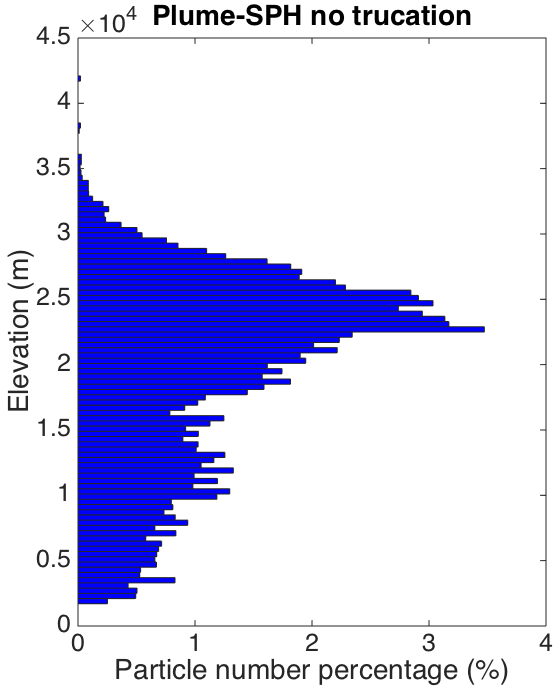
\includegraphics[width=0.99 \textwidth]{Chapter-7/Figures/Plume-SPH-ParticleDis-NoTrucation-z}
    \end{minipage}%
    \begin{minipage}{.247 \textwidth}
        \centering
        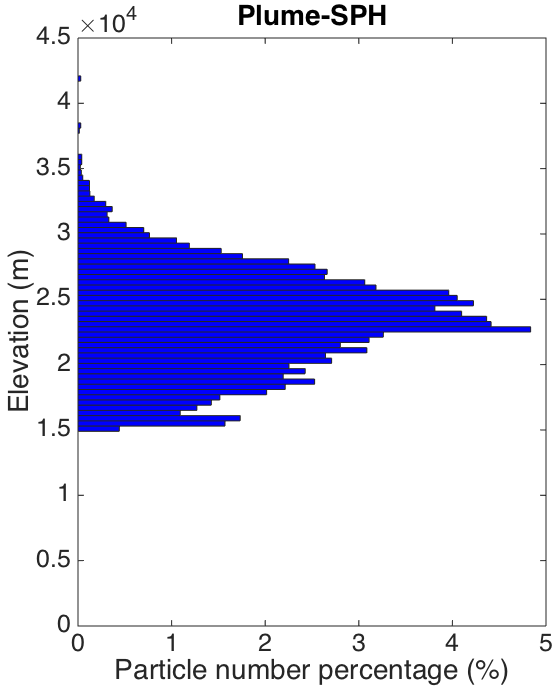
\includegraphics[width=0.99 \textwidth]{Chapter-7/Figures/Plume-SPH-ParticleDis-z}
    \end{minipage}%
    \begin{minipage}{.247 \textwidth}
        \centering
        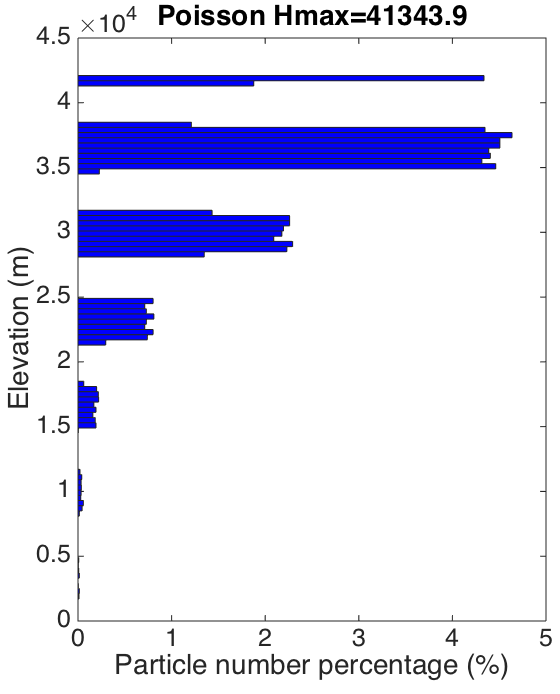
\includegraphics[width=0.99 \textwidth]{Chapter-7/Figures/Possion-Hmax40k-ParticleDis-z}
    \end{minipage}% 
    \begin{minipage}{.247 \textwidth}
        \centering
        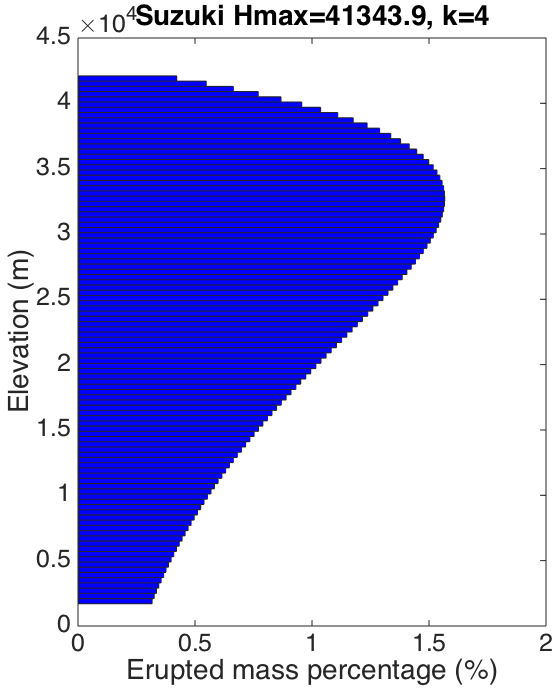
\includegraphics[width=0.99 \textwidth]{Chapter-7/Figures/Suzuki-Hmax40k-ParticleDis-z}
    \end{minipage}% 
    \caption{Particle distribution of initial ash cloud in vertical direction. The picture to the left is corresponding to initial ash cloud obtained from Plume-SPH output. The second picture is corresponding to ash distribution truncated by a elevation threshold of $15000 m$. Third picture is corresponding to Poisson distribution with maximum height based on bent simulation. Another parameter, the vertical spread, in the expression of Poisson plume shape is $6662 m$. The picture to the right is corresponding to Suzuki distribution with maximum height based on bent simulation. Another parameter in Suzuki distribution, the shape factor, is $4$. The $x$ axis is the percentage of particle number for Plume-SPH and Poisson, is the percentage of erupted material mass percentage for Suzuki.}
    \label{fig:Particle-distribution-Plume-SPH-vs-semiempirical}
\end{figure}

For Poisson and Suzuki plume shape, vertical distribution of ash particles can't be lower down without changing the maximum height. To distribute majority population of ash particles at lower elevation, the maximum height has to be reduced to a value smaller than observed maximum height. This strategy is the same as the traditional source term calibration method. A set of initial ash clouds using different maximum heights based on Poisson plume shape assumption is shown in Fig. \ref{fig:Particle-distribution-Plume-calibrate-semiempirical}). The maximum heights, by no means, are obtained from any plume model or observation. Except for maximum height, all other parameters for creating initial ash cloud are the same as these in Table \ref{tab:input_parameter_PUFF_simulation}. The range between which major populations of ash particles locate is different when using different maximum heights. These ash clouds based on different maximum heights are then used as initial condition in PUFF simulation. The ash transportation simulation results with initial condition based on different maximum height are show in Fig. \ref{fig:Various-Maximum-height-Pinatubo-ash-cloud}.

\begin{figure}[!htb]
    \centering
    \begin{minipage}{.247 \textwidth}
        \centering
        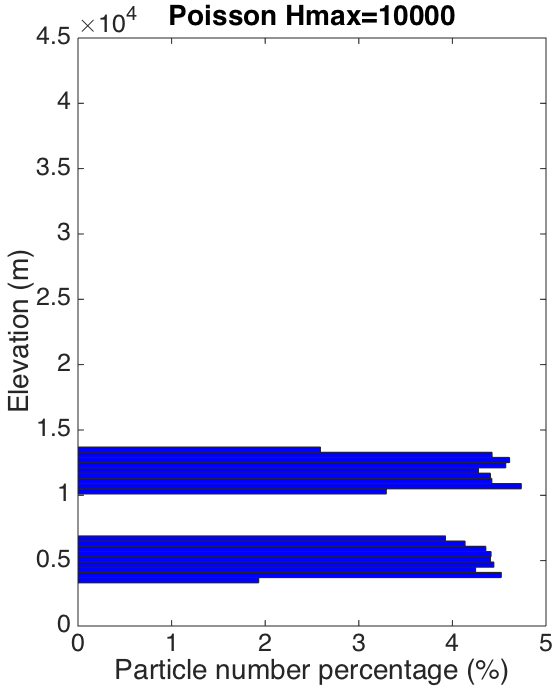
\includegraphics[width=0.99 \textwidth]{Chapter-7/Figures/Possion-Hmax10k-ParticleDis-z}
    \end{minipage}%
    \begin{minipage}{.247 \textwidth}
        \centering
        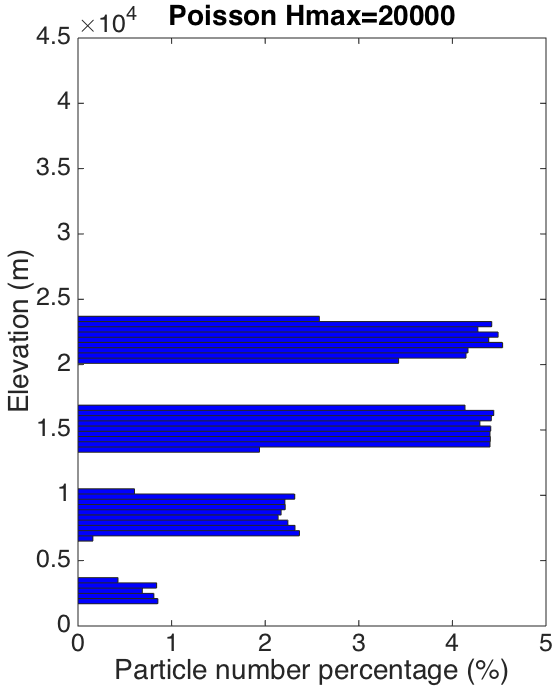
\includegraphics[width=0.99 \textwidth]{Chapter-7/Figures/Possion-Hmax20k-ParticleDis-z}
    \end{minipage}% 
    \begin{minipage}{.247 \textwidth}
        \centering
        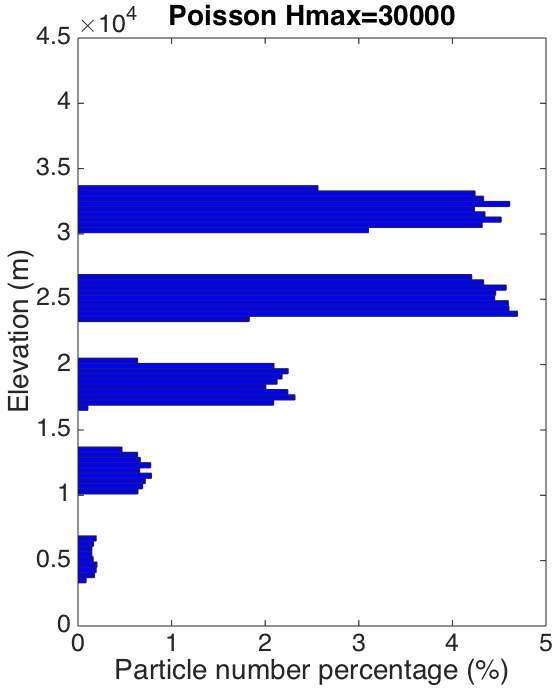
\includegraphics[width=0.99 \textwidth]{Chapter-7/Figures/Possion-Hmax30k-ParticleDis-z}
    \end{minipage}% 
    \begin{minipage}{.247 \textwidth}
        \centering
        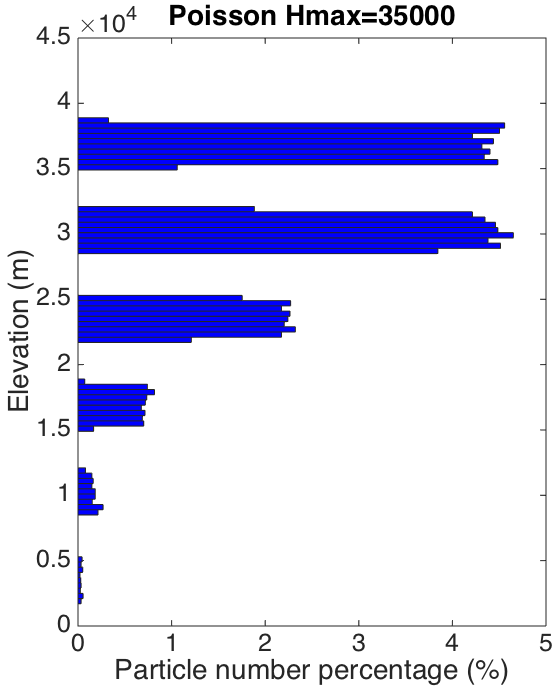
\includegraphics[width=0.99 \textwidth]{Chapter-7/Figures/Possion-Hmax35k-ParticleDis-z}
    \end{minipage}% 
    \caption{Particle distribution based on Poisson plume shape in vertical direction with different maximum heights. Pictures from left to right are corresponding to maximum height of $10000 m$,  $20000 m$,  $30000 m$, $35000 m$. Another parameter, the vertical spread, in the expression of Poisson plume shape is $6662 m$ for all cases. The $x$ axis is the percentage of particle number.}
    \label{fig:Particle-distribution-Plume-calibrate-semiempirical}
\end{figure}

\begin{figure}[!htb]
    \centering
    \begin{minipage}{.245\textwidth}
        \centering
        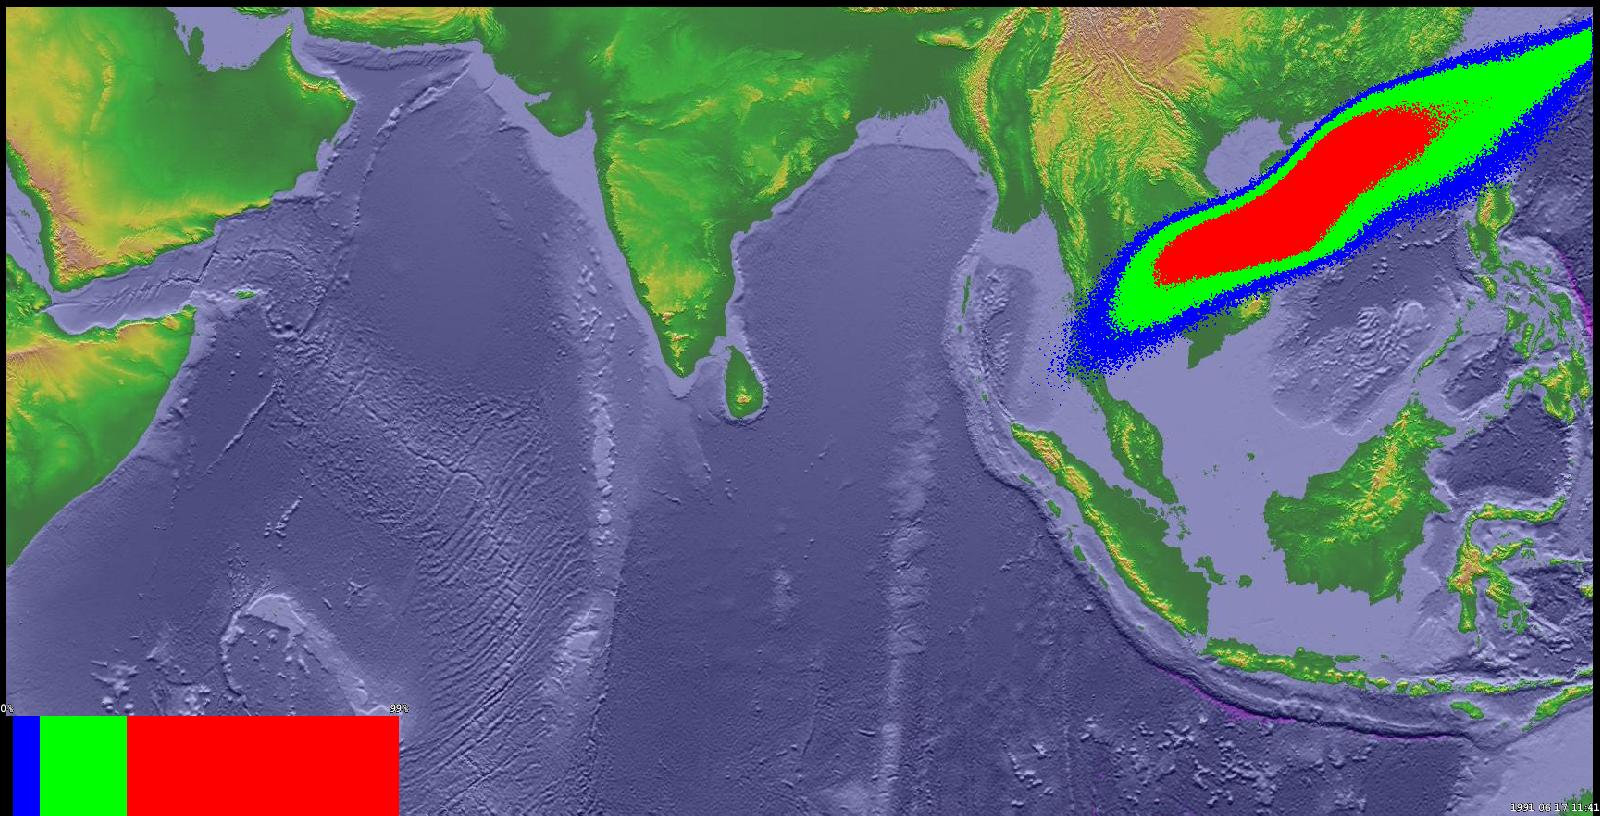
\includegraphics[width=0.99 \textwidth]{Chapter-7/Figures/bent-55hr-ash-MaxH10000}
    \end{minipage}%
    \begin{minipage}{.245 \textwidth}
        \centering
        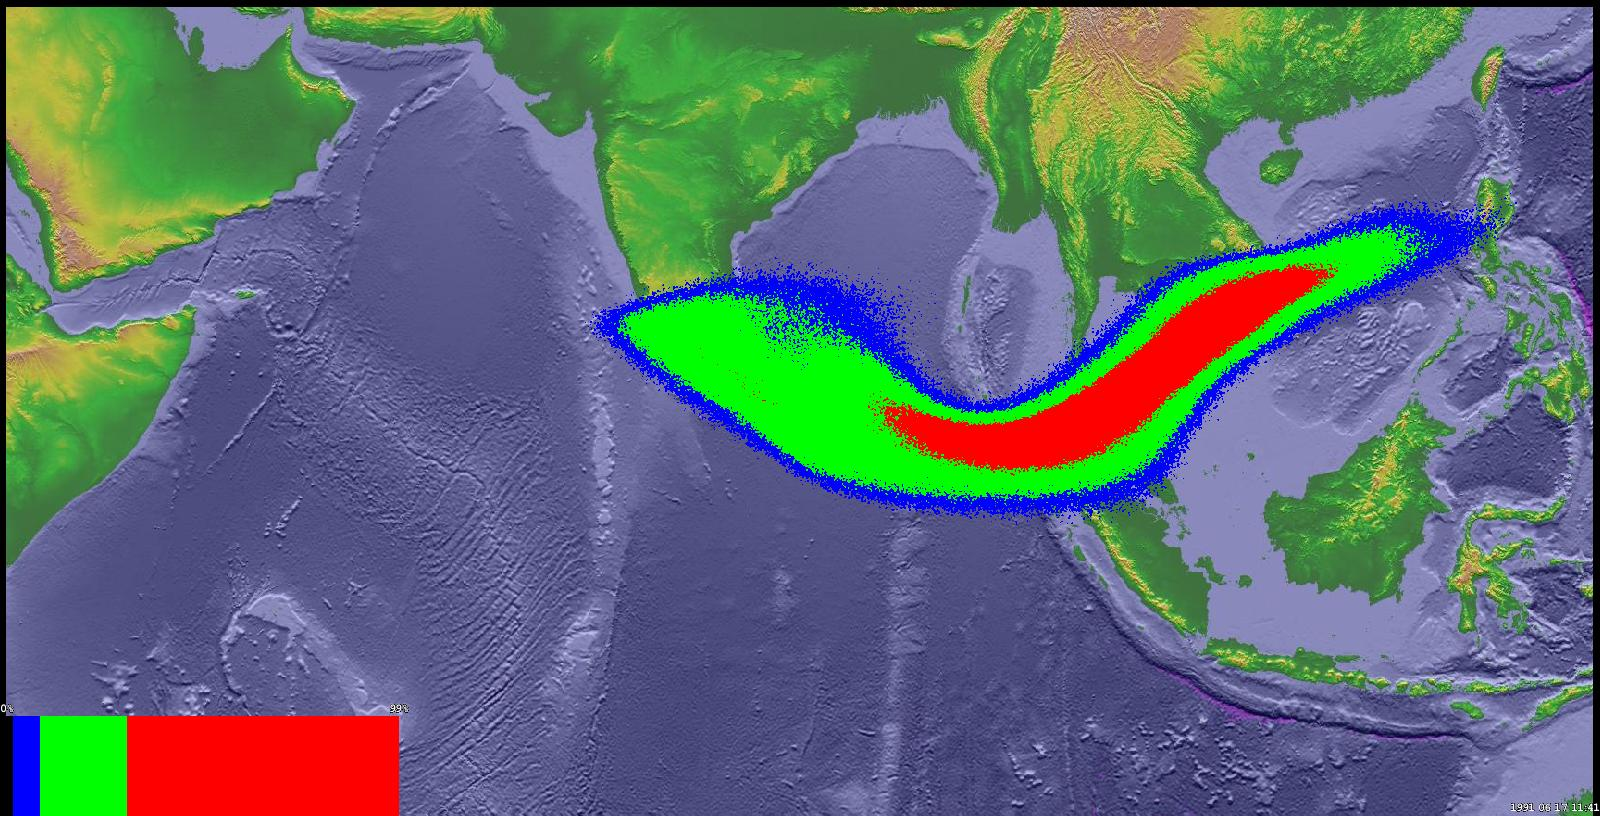
\includegraphics[width=0.99 \textwidth]{Chapter-7/Figures/bent-55hr-ash-MaxH20000}
    \end{minipage}%
    \begin{minipage}{.245 \textwidth}
        \centering
        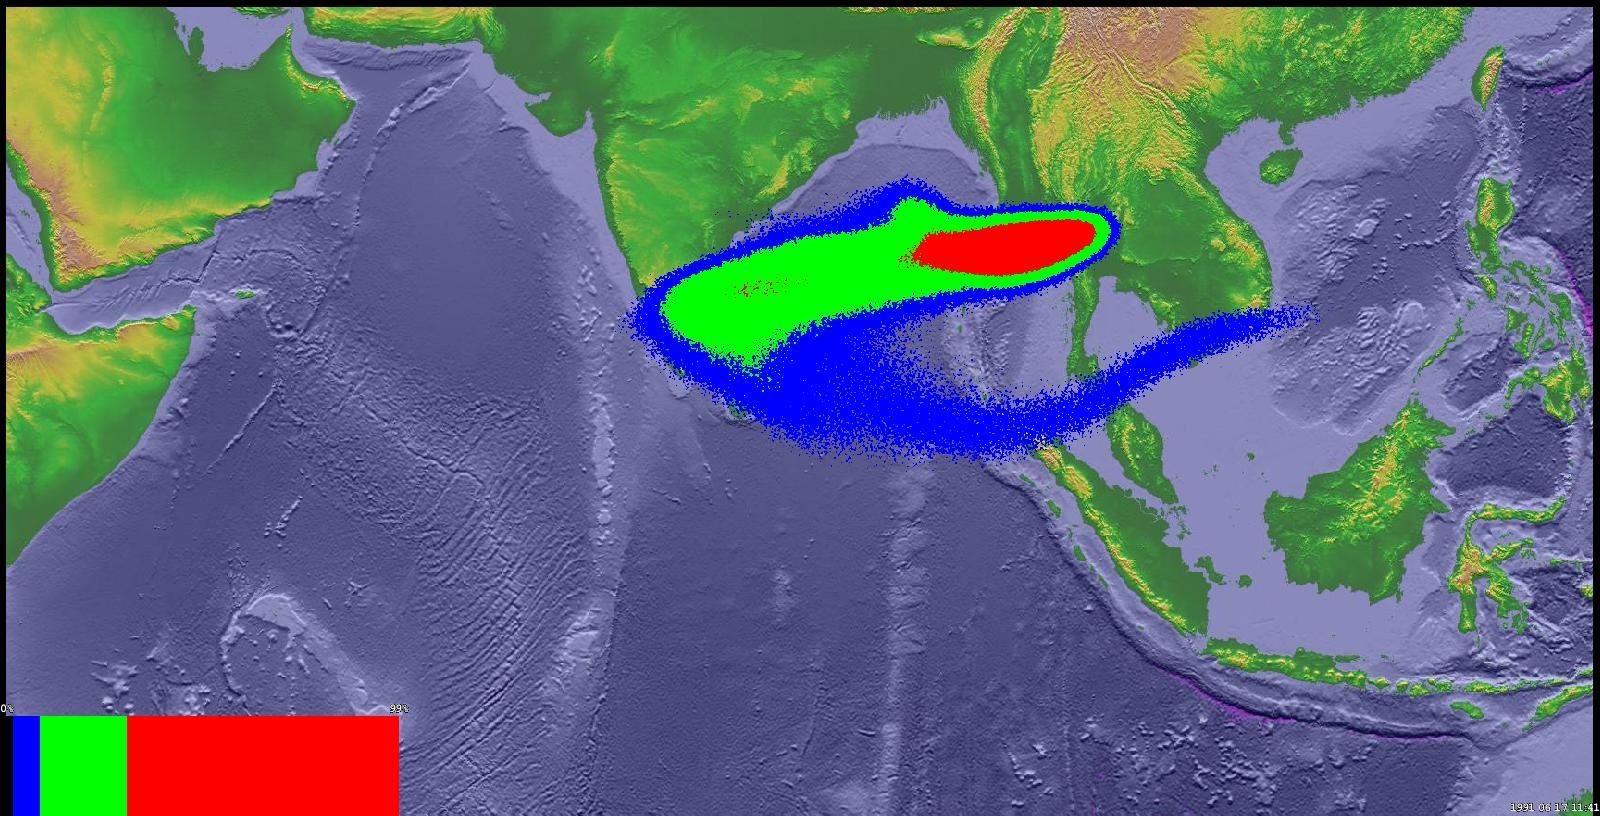
\includegraphics[width=0.99 \textwidth]{Chapter-7/Figures/bent-55hr-ash-MaxH30000}
    \end{minipage}%  
    \begin{minipage}{.245 \textwidth}
        \centering
        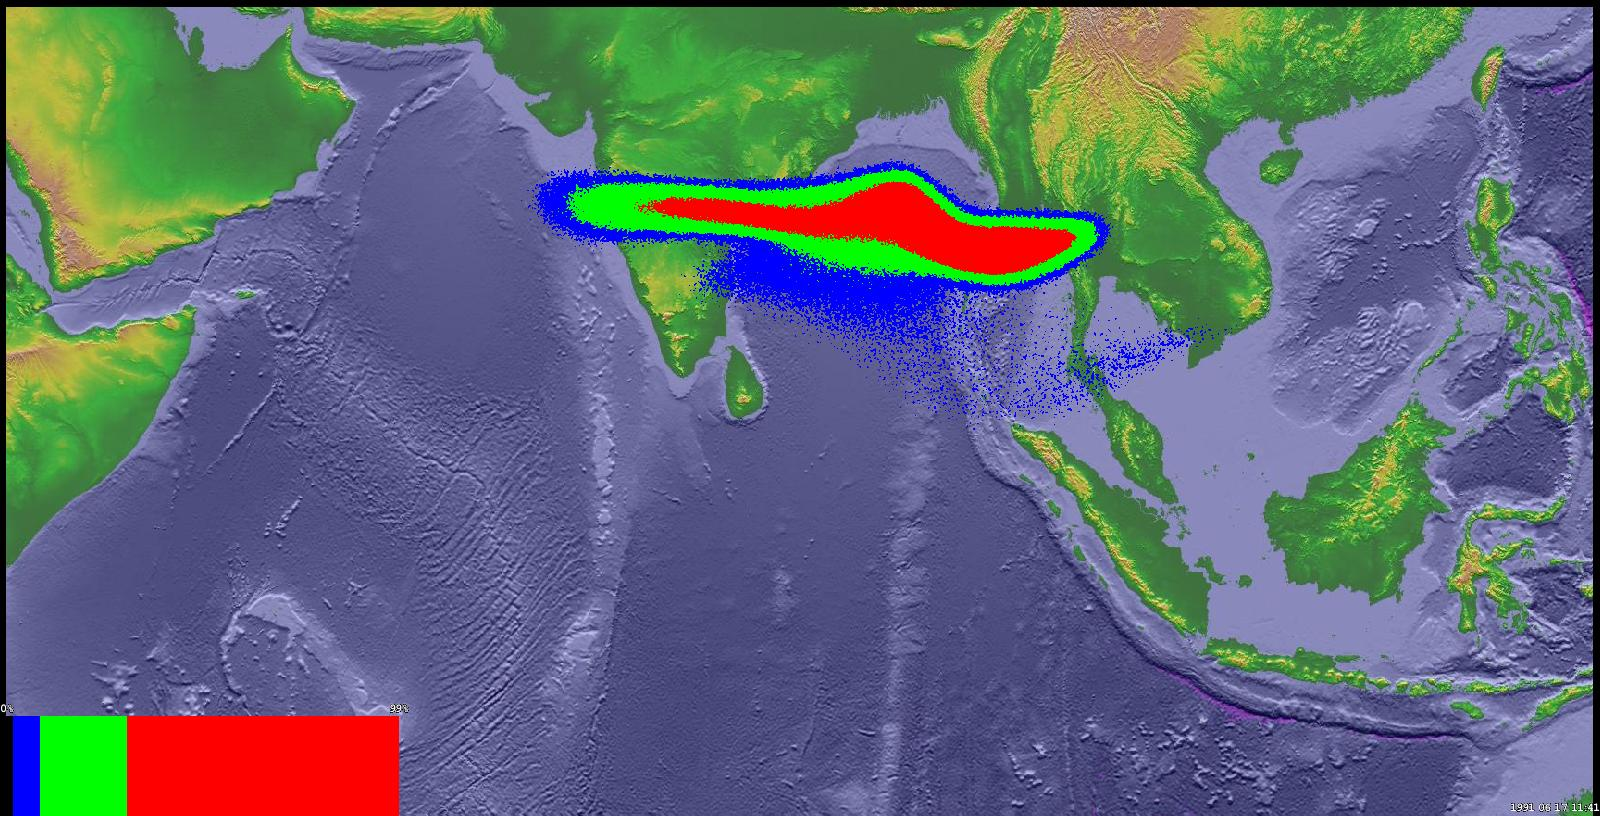
\includegraphics[width=0.99 \textwidth]{Chapter-7/Figures/bent-55hr-ash-MaxH35000}
    \end{minipage}%   
    \caption{Ash transportation simulated by PUFF using different initial ash cloud created with different maximum heights. Pictures from left to right are: PUFF simulation with maximum plume height of $10000 m$, $20000 m$, $30000 m$ and $35000 m$. The images are corresponding to around 55 hours after eruption (UT 199106171141).  See the observed cloud image in Fig. \ref{fig:Plume-SPH-PUFF-ash-cloud}. }
    \label{fig:Various-Maximum-height-Pinatubo-ash-cloud}
\end{figure}

Figure \ref{fig:Various-Maximum-height-Pinatubo-ash-cloud} shows that the maximum height has significant influence on ash transportation simulation. When the maximum height is $10000 m$ or $20000 m$, the high concentration area is lag behind observation. While the designated maximum height is $35000 m$, the high concentration area is a little bit faster and much narrower than observation. When using maximum height of $41343.9 m$, the high concentration area is faster and narrower (see Fig. \ref{fig:Plume-SPH-PUFF-ash-cloud}) than those of the simulation results based on maximum height of $35000 m$. The simulated high concentration area is closest to observation when assigning a maximum height of $30000 m$. The front of volcano ash, with lower concentration, locates west to high concentration area. A lower concentration tailing area also appears in the simulation results while there is no such tail in observed image. PUFF simulation result based on calibrated maximum height of $30000 m$ shows similar footprint to, even though smaller in terms of covered area than, those of ``Pume-SPH+PUFF" simulation. We conclude that, for climactic phase of Pinatubo eruption, the initial ash cloud created with maximum height around 30000 m generates best match ash distribution with observation. That is to say, a maximum height lower than real maximum height of plume is required by Poisson plume shape to distribute ash particles at the same elevation as real ash distribution. Our hypothesis regarding the source of disparity between "bent+PUFF" simulation and observation is confirmed.

In this section, only maximum height is adjusted to obtain more realistic ash distribution. Other parameters that also control the plume shape, such as such as vertical spread and plume width, if calibrated properly, could generate an initial ash cloud that closer to real one. However, the degree of freedom to adjust plume shape might still be limited. 3D plume models, which can generate 3D initial ash cloud without any assumption about plume shape, provide an alternative way for creating initial conditions.

\subsection{$SO_2$ clouds}
In terms of long-term ash transportation simulation, for example, two days after climactic phase starts, ash distribution simulated by ``Plume-SPH+PUFF" are faster and wider spread than observation. Several factors could contribute to the disparity between simulation and real distribution. Such as simplification in physics model, numerical error, initial condition and boundary conditions. We suspect that the disparity between simulation and observation of long-term ash transportation are majorly attributed to the simplification in PUFF, in which no microphysics is considered. PUFF takes into account the predominant physical processes that control particle movement, such as winds, dispersion and settling, but it does not account for small scales physical processes. However, the microphysics, especially the mixed aggregation of ice and ash particles has been reported to enhance fallout \citep{guo2004particles} of Pinatubo ash particles. Thereby, both ice and ash particles declined very rapidly within 3 days. Without considering the effect of mixed aggregation due to presence of ice, PUFF did poor job in long-term ash transportation forecast of Pinatubo eruption.

The physics model of PUFF underestimates fallout of particles in scenarios when ice presents. The presence of ice, however, has less influence on $SO_2$ transportation. That is to say, PUFF might be used to simulate long-term $SO_2$ transportation, even though it was originally developed for volcanic ash transportation. The settling accounted in PUFF might be viewed as "mass sink" of $SO_2$ due to, for example, absorption or chemical reaction. More rigorous "mass sink" needs to be developed to adapt PUFF to be a real $SO_2$ cloud transportation model. In this section, we roughly use PUFF for $SO_2$ simulation to investigate why we observe more obvious disparity between simulation and observation of long-term ash distribution. 

\begin{figure}[!htb]
    \centering
    \begin{minipage}{.325\textwidth}
        \centering
        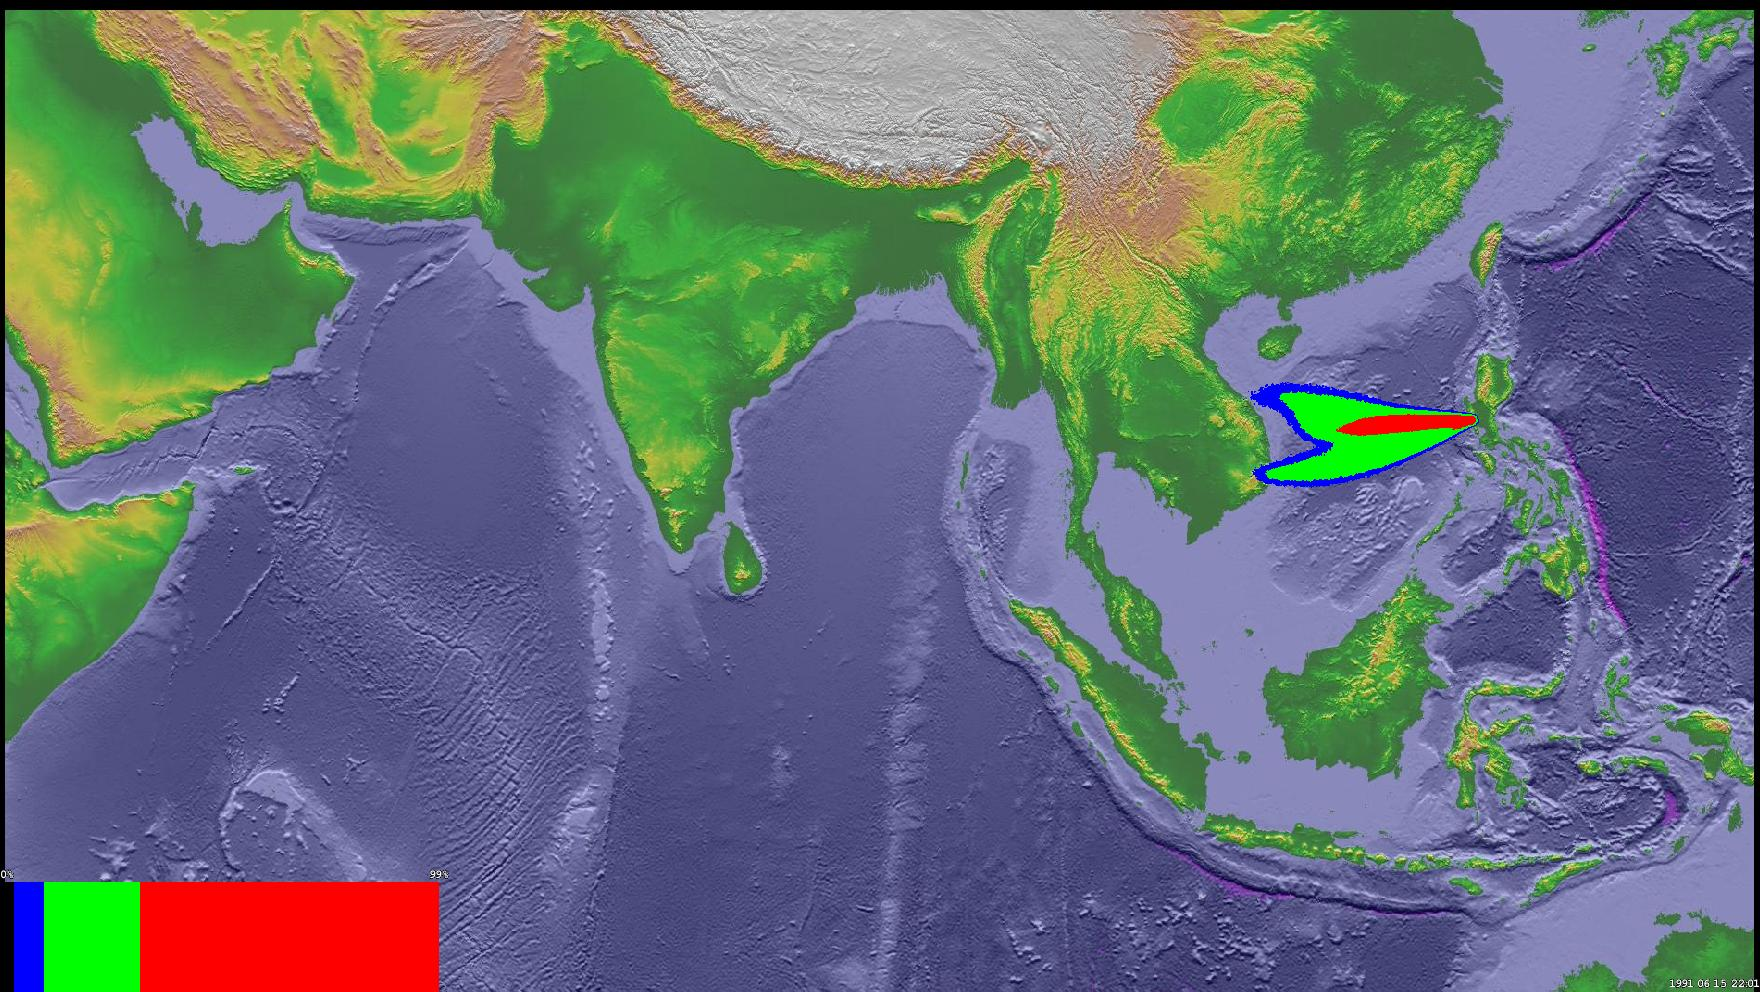
\includegraphics[width=0.99 \textwidth]{Chapter-7/Figures/SPH-Plume-7p3hr-ash}
    \end{minipage}%
    \begin{minipage}{.325 \textwidth}
        \centering
        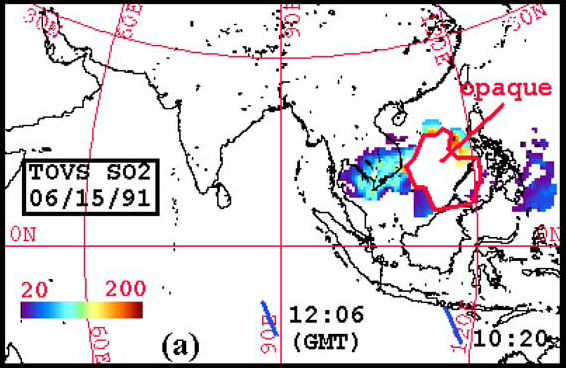
\includegraphics[width=0.99 \textwidth]{Chapter-7/Figures/OB-SO2-7p3hr-ash}
    \end{minipage}% 
    \\
    \begin{minipage}{.325\textwidth}
        \centering
        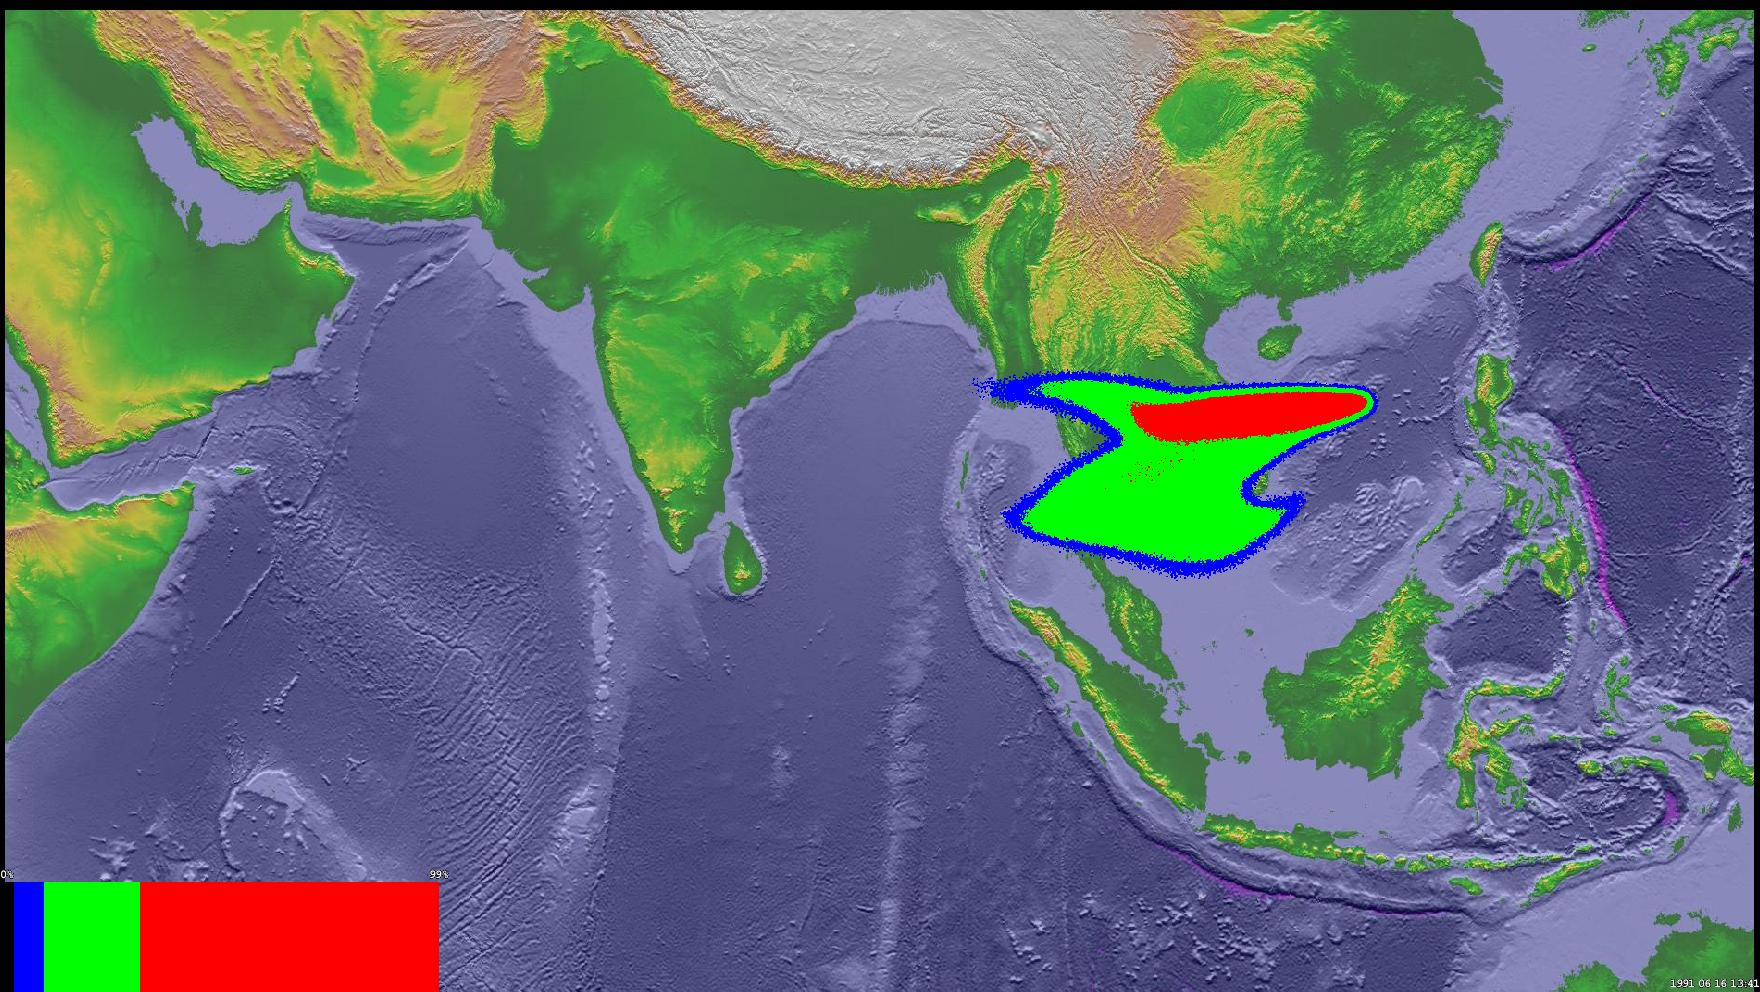
\includegraphics[width=0.99 \textwidth]{Chapter-7/Figures/SPH-Plume-23hr-ash}
    \end{minipage}%
    \begin{minipage}{.325 \textwidth}
        \centering
        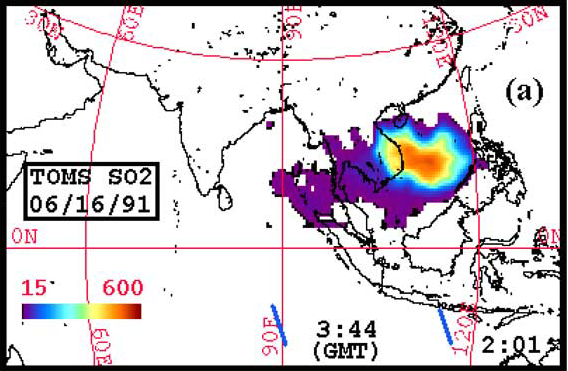
\includegraphics[width=0.99 \textwidth]{Chapter-7/Figures/OB-SO2-23hr-ash}
    \end{minipage}% 
    \\
    \begin{minipage}{.325\textwidth}
        \centering
        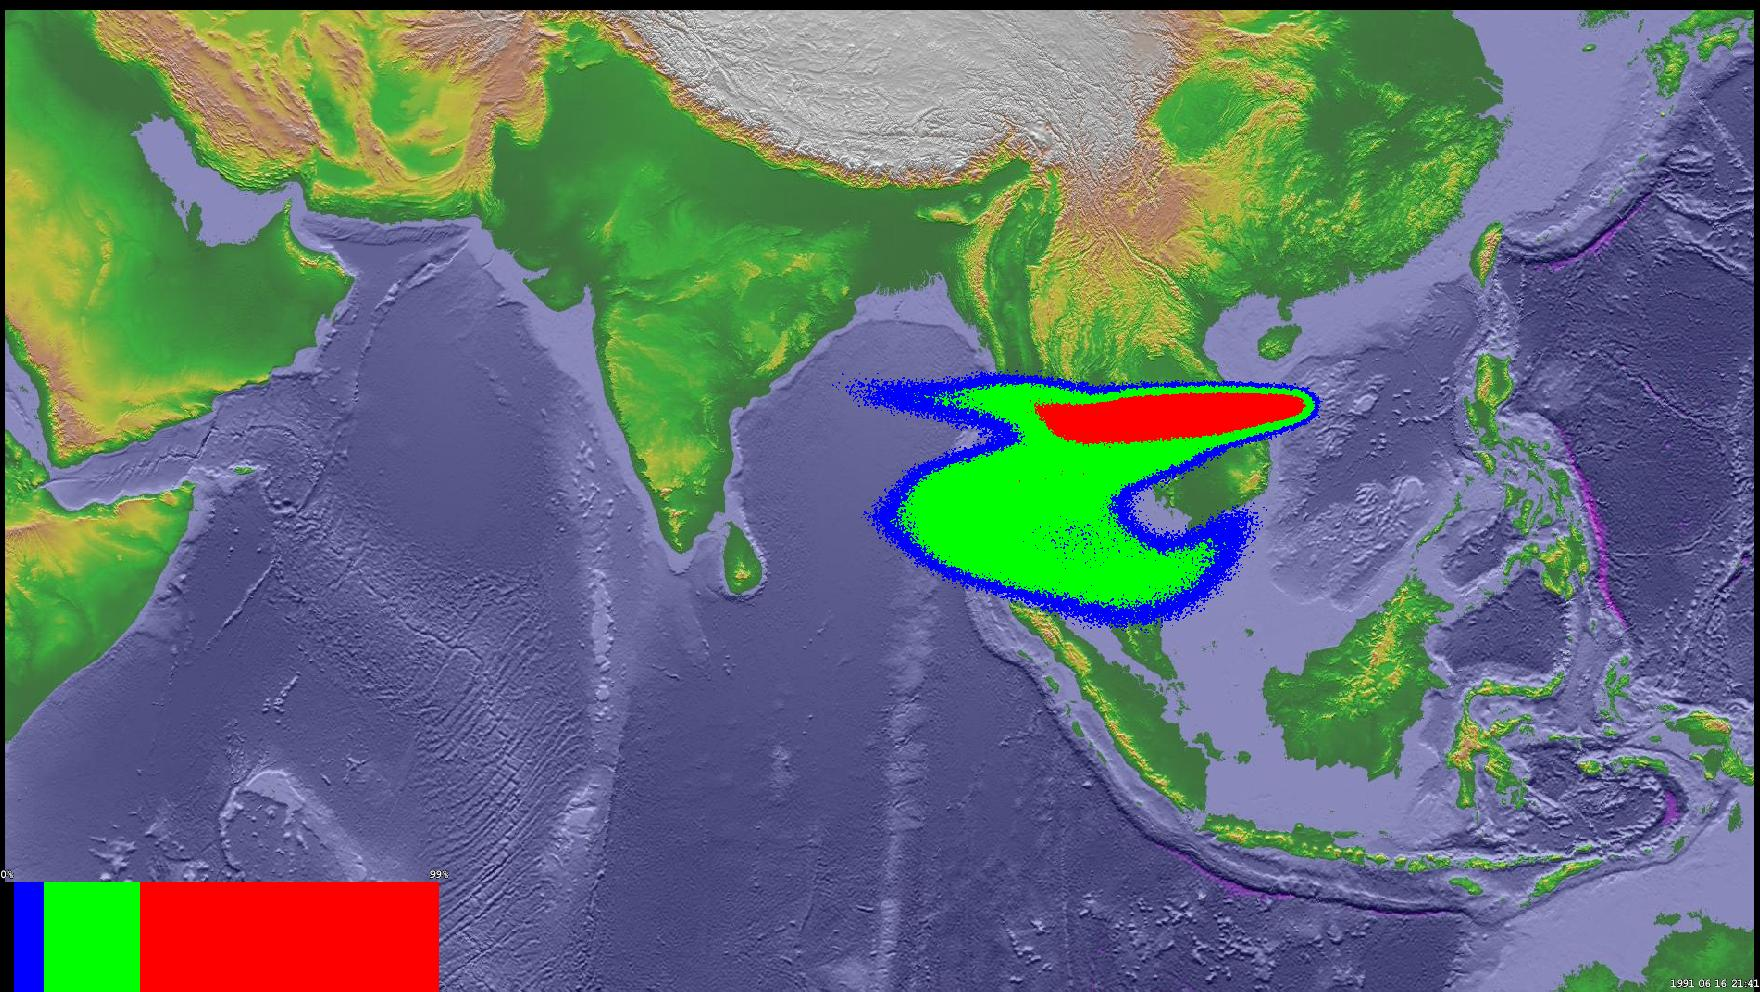
\includegraphics[width=0.99 \textwidth]{Chapter-7/Figures/SPH-Plume-31hr-ash}
    \end{minipage}%
    \begin{minipage}{.325 \textwidth}
        \centering
        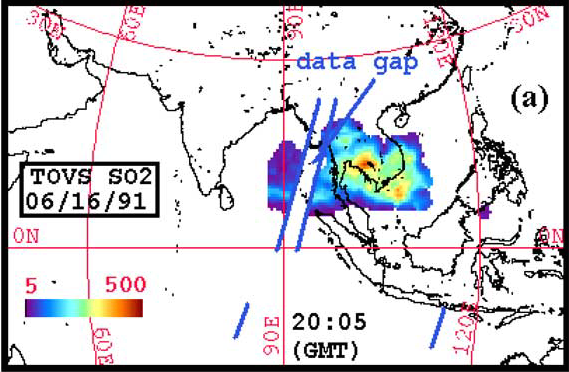
\includegraphics[width=0.99 \textwidth]{Chapter-7/Figures/OB-SO2-31hr-ash}
    \end{minipage}% 
\\
    \begin{minipage}{.325\textwidth}
        \centering
        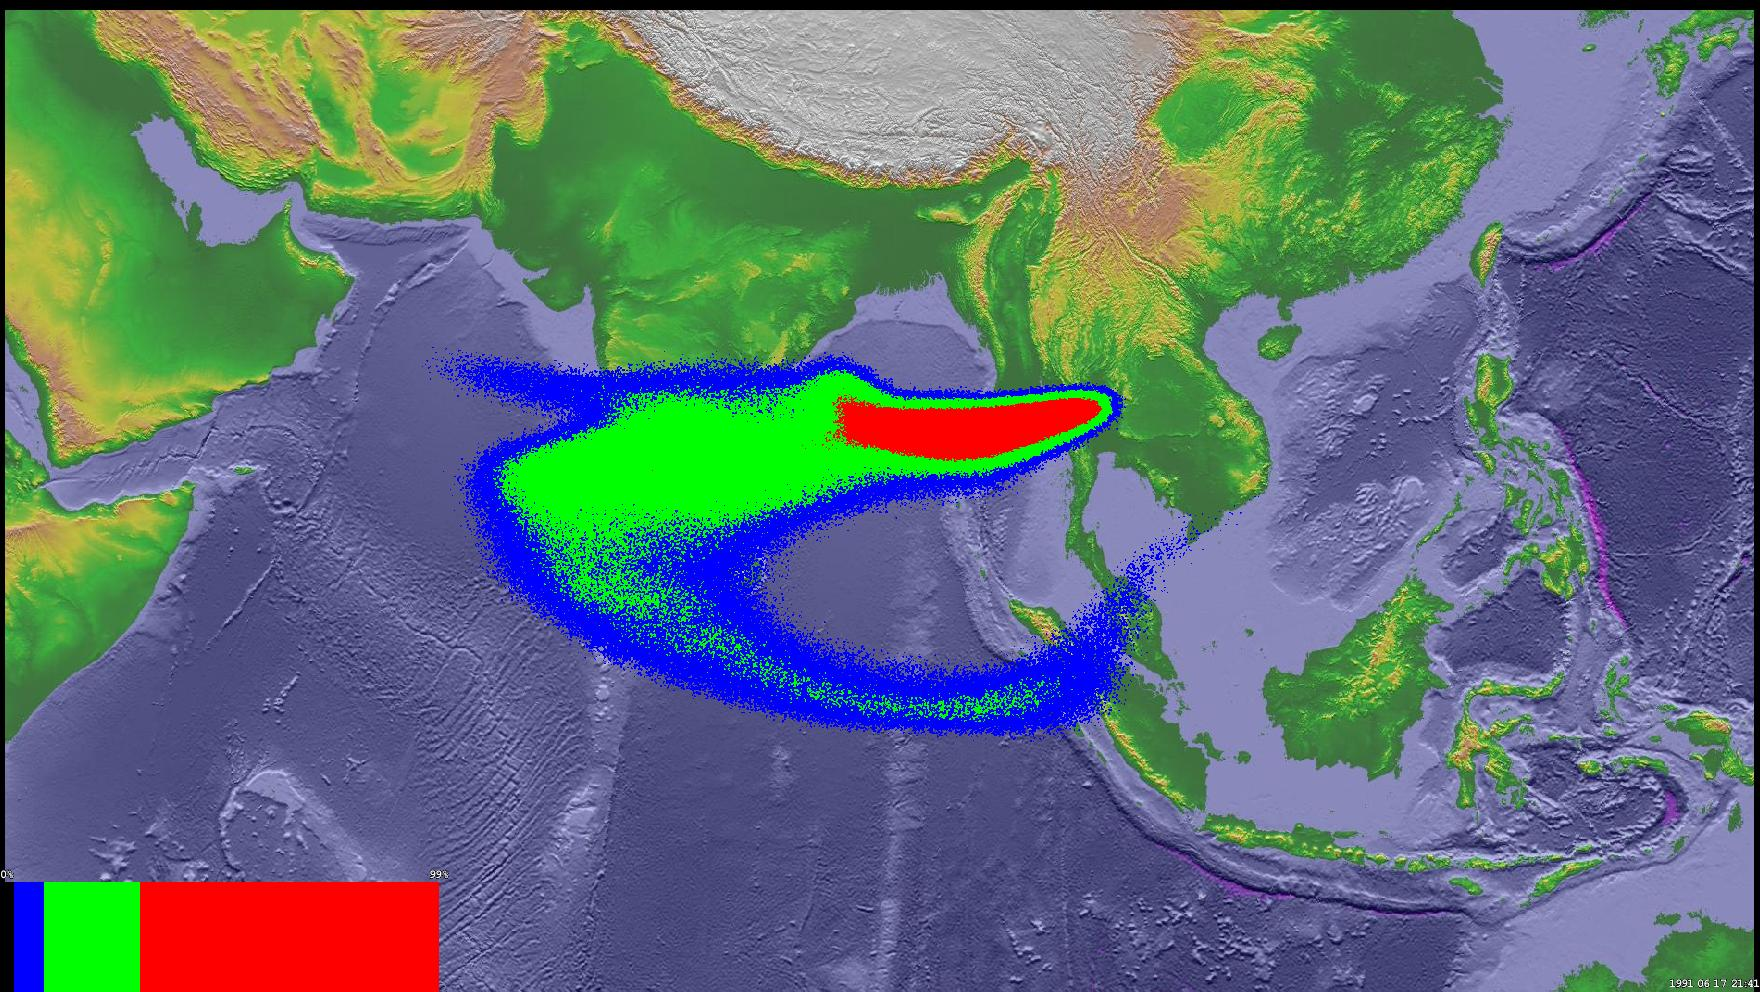
\includegraphics[width=0.99 \textwidth]{Chapter-7/Figures/SPH-Plume-55hr-ash}
    \end{minipage}%
    \begin{minipage}{.325 \textwidth}
        \centering
        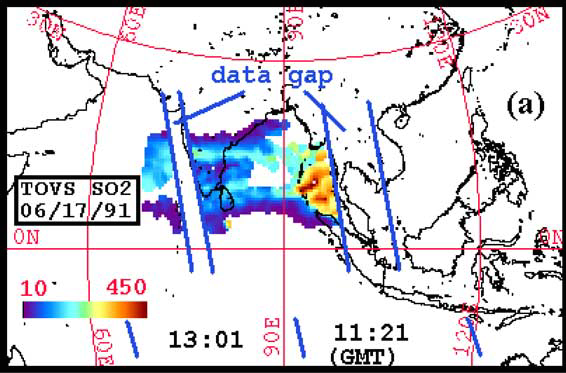
\includegraphics[width=0.99 \textwidth]{Chapter-7/Figures/OB-SO2-55hr-ash}
    \end{minipage}% 
\\
    \begin{minipage}{.325\textwidth}
        \centering
        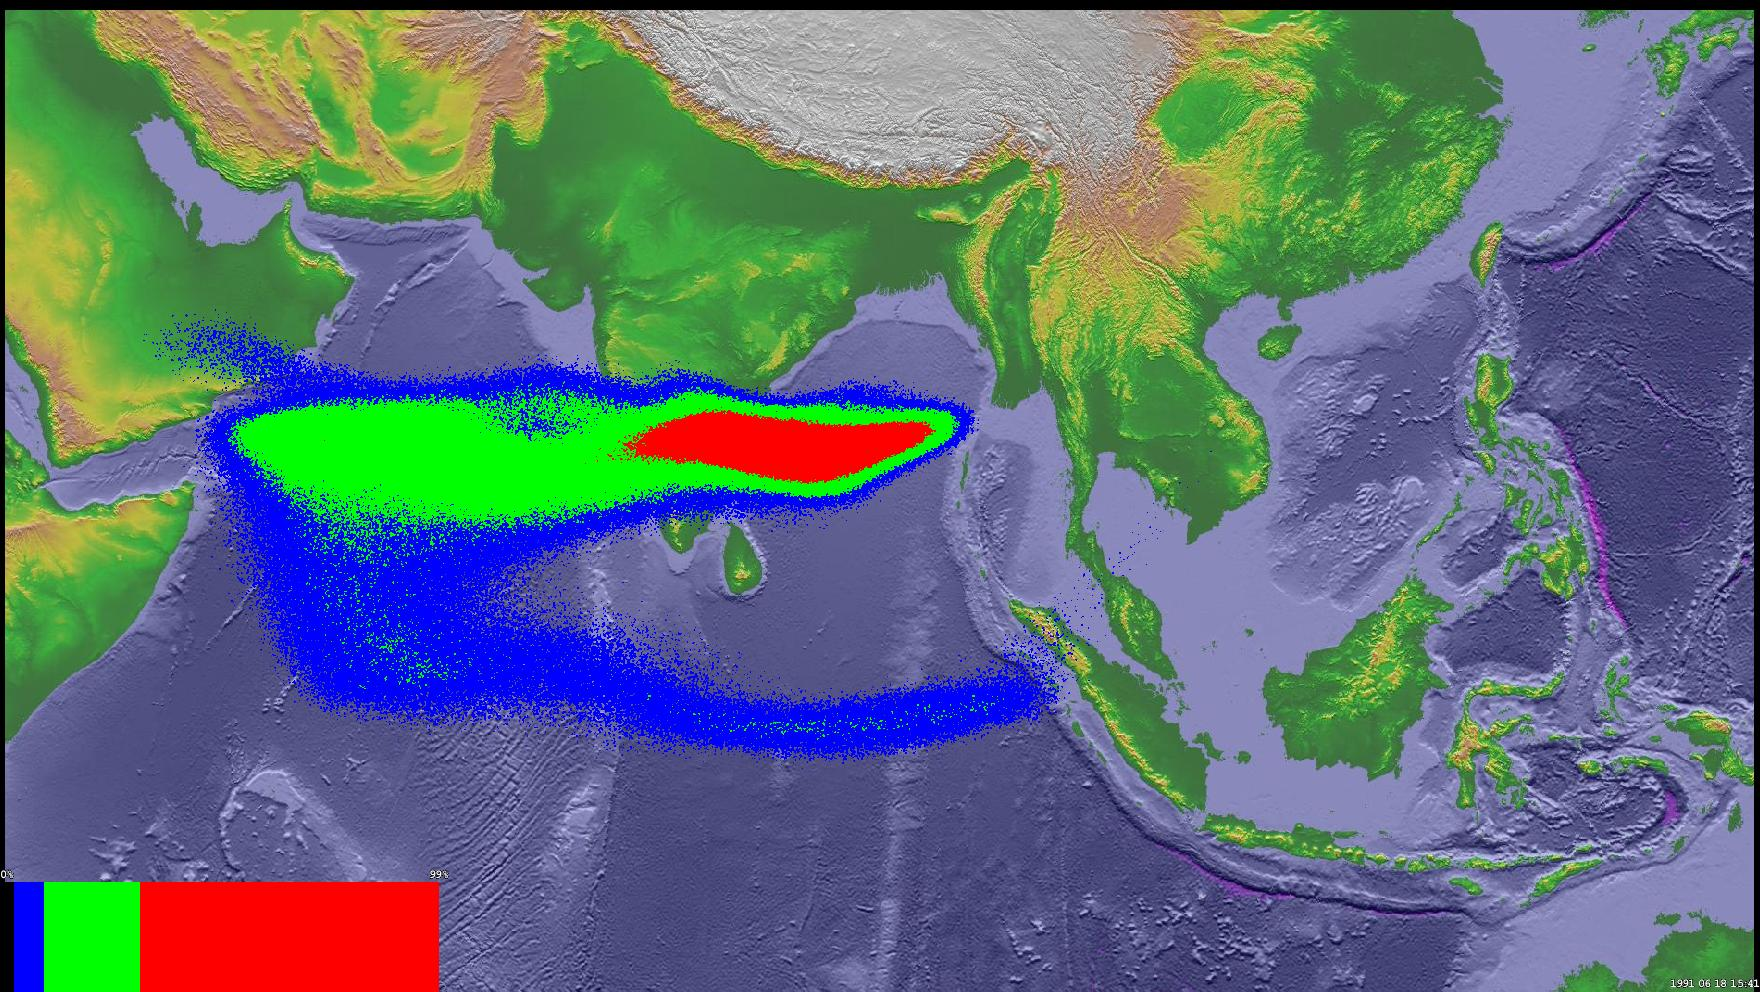
\includegraphics[width=0.99 \textwidth]{Chapter-7/Figures/SPH-Plume-73hr-ash}
    \end{minipage}%
    \begin{minipage}{.325 \textwidth}
        \centering
        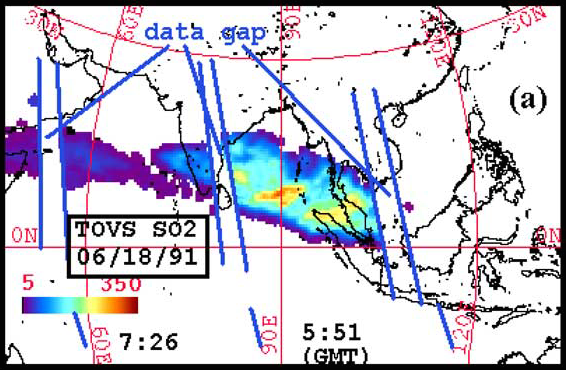
\includegraphics[width=0.99 \textwidth]{Chapter-7/Figures/OB-SO2-73hr-ash}
    \end{minipage}% 
    \caption{Comparison of volcanic clouds simulated by ``Plume-SPH+PUFF" and observed $SO_2$ cloud. Pictures to the left are PUFF simulation based on Plume-SPH, pictures on the right are TOMS or AVHRR image of Pinatubo $SO_2$ cloud. $SO_2$ clouds at different hours after eruption are on different rows. From top to bottom, the images are corresponding to around 7.3 hours after starting of climatic phase (UT 199106151201), 23 hours after starting of climatic phase (UT 199106160341), 31 hours after starting of climatic phase (UT 199106161141), 55 hours after starting of climatic phase (UT 199106171141), 73 hours after starting of climatic phase (UT 199106180541).}
    \label{fig:Plume-SPH-Pinatubo-SO2-cloud}
\end{figure}

We observe in Fig. \ref{fig:Plume-SPH-Pinatubo-SO2-cloud} that the simulated ash distribution match well with observed $SO_2$ cloud after more than one day since the beginning of climactic phase. At around 7.3 hours and 21 hours after eruption, the observed $SO_2$ ash covers a obviously large area. This is due to the fact that our simulation is only for the climactic phase but satellite observation includes $SO_2$ clouds existing before the climactic phase. At around 31 hours after starting of climactic phase, the simulated cloud match well with observation. The location of high concentration area in simulation is also consistent with observation. At 55 hours and 73 hours after starting of climactic phase, the front of simulated volcano cloud is close to observation, while the tail of simulated volcano cloud locate west to the observed tail. The area of high concentration also locates to the west of observed high concentration area. Considering that Pinatubo continued eruption after climactic phase, it is understandable that tail of observed $SO_2$ clouds is at east to the simulated tail. To reduce such disparity, the eruption duration for PUFF should be extended to include pre-climactic phase and post-climactic phase. Of course, the initial ash cloud corresponding to pre-climactic phase and post-climactic phase should be different from that of climactic phase.

To conclude, the obvious disparity between observation and PUFF simulation results of long-term ash transportation is due to inability of PUFF in accounting for acceleration of ash settling caused by ice. More physics, such as the ice caused acceleration of ash particle settling, should be included so that PUFF is able to account for aggregation and predict fallout in a more accurate way. A source term, which represents losing of $SO_2$ during transportation, is necessary to extend PUFF to a $SO_2$ transportation model.

\section*{Conclusion}

In this paper, we presented, for the first time, a new methodology to create initial conditions for volcanic ash transportation and dispersal simulation. The new method extracts initial ash cloud from 3D plume simulation while traditional methods create initial ash cloud based on semiemperical plume shape expression. Case study of Pinatubo eruption demonstrates that this new method can create more realistic initial ash cloud and improve accuracy of ash transportation forecast. In order to explain why we got much closer ash dispersal forecast merely by adopting new initial conditions, more investigations were conducted. Sensitivity analyses illustrate that initial condition has more significant effects on volcanic ash transportation forecast than most of the other input parameters. Calibrating of the maximum height in semiemperical plume shape expression reveals how vertical ash particle distribution in initial ash cloud could affect ash transportation forecast. At the end, the disparity between simulation and observation of long-term ash transportation is investigated concluding that it is necessary for VATDs to account for aggregation due to ice to reduce disparity in Pinatubo ash transportation forecast.

This new method provides an alternative option for creating initial conditions for ash transportation simulations. Except for the disadvantage of high computational cost it helps overcome several shortcomings of existing methods.
As numerical models based on first principle, 3D plume models eliminate parameterization and hence user intervention associated with entrainment coefficients. Thereby, obtaining initial conditions from 3D plume models could improve forecast capacity of ash transportation simulation. More importantly, with output in 3D space, no assumption about plume shape needed. The plume shape generated directly by 3D simulation is more realistic and adaptive to various scenarios.
Contrastingly, semiempirical plume shape expressions only have several parameters control the shape of initial ash cloud, it might have difficulties to generate initial ash cloud that close to reality for some eruptions.
For the case study of Pinatubo eruption, we got closer simulation results to observation when using maximum height of around $30 km$, which is much lower than observed plume height of $40 km$. It is evidence that initial ash cloud created according to semiempirical plume shape would be discrepant from real one for some eruptions. As has been shown by sensitivity analyses, such disparity has much greater influence on ash evolution simulation than all other input parameters.

The full range of research issues raised by the numerical forecasting of volcanic clouds is many and diverse. We described in this paper the effect of initial conditions on numerical forecasts of volcanic ash transportation simulation, especially the effects of vertical ash particles distribution in the initial ash cloud. 
In fact, the difference between assumed plume particle distribution and actual (or simulated by 3D plume) model is not only in vertical direction. How do other aspects of particle distribution in the initial ash cloud affect ash transportation is yet to explore. Wind field, another important factor in volcanic ash transportation simulation is not discussed in this paper, either. Some other aspects, such as small scale physical processes, even though plays less roles, might need to be included by VATDs to improve accuracy. In addition, the eruption condition, hence the initial ash clouds are subject to change during eruption, even during climactic phase of eruption. More realistic initial condition for VATDs can be created from 3D plume simulation with time-dependent eruption conditions.